\documentclass[english,11pt]{article}
\usepackage[paperwidth=210mm,paperheight=297mm,margin=15mm]{geometry}
%\usepackage{algorithmic,algorithm}
\usepackage{psfrag,subfigure}
\usepackage{epsfig,multirow,color,url,colortbl,xcolor}
\usepackage[latin1]{inputenc}
\usepackage{amssymb,fancyhdr,epsfig,psfrag,tabularx,amsmath,theorem,pifont}
\usepackage[brazil]{babel}
%\usepackage{matlab-prettifier}
% Build from docs/ with latexmk -pdfps -jobname=manual_rolmip rolmip_manual.tex.
% The DVI/PostScript route preserves the psfrag labels in the EPS figures.
\graphicspath{{manual_assets/}}
\usepackage[bw,framed]{mcode}
\usepackage[hidelinks,bookmarks=false]{hyperref}

\lstset{breaklines=true,breakatwhitespace=false}
\lstdefinestyle{ManualCode}{basicstyle=\lstbasicfont,
  keywordstyle=\bfseries,commentstyle=\itshape,
  stringstyle=\color{black},rulecolor=\color{black}}

\newcommand*{\colorboxed}{}
\def\colorboxed#1#{%
  \colorboxedAux{#1}%
}
\newcommand*{\colorboxedAux}[3]{%
  % #1: optional argument for color model
  % #2: color specification
  % #3: formula
  \begingroup
    \colorlet{cb@saved}{.}%
    \color#1{#2}%
    \boxed{%
      \color{cb@saved}%
      #3%
    }%
  \endgroup
}

% configuration of tables with gray background
\definecolor{gray1}{gray}{0.95}
\newcolumntype{A}{>{\columncolor{gray1}}c}
\definecolor{defbkgd}{gray}{0.95}
\doublerulesepcolor{defbkgd}


\newcommand\hi{\hspace*{\parindent}}
\newcommand\vi{\vspace{.5cm}}


\theoremstyle{break} \theorembodyfont{\small\rm}
\newtheorem{exemplo}{\bf Example}

\theorembodyfont{\rm}
\newtheorem{propri}{\bf Property}

\theorembodyfont{\rm}
\newtheorem{teorema}{\bf Theorem}

\theorembodyfont{\rm}
\newtheorem{definicao}{\bf Definition}

\theorembodyfont{\rm}
\newtheorem{rem}{\bf Remark}

\theorembodyfont{\rm}
\newtheorem{lema}{\bf Lemma}

\theorembodyfont{\rm}
\newtheorem{algorithm}{\bf Algorithm}

\newcounter{Iexctr}
\newenvironment{Iexemplo}[1]
{\stepcounter{Iexctr} \begin{center} \begin{quote} \small {\bf
Exemplo~\arabic{Iexctr}: {#1}} \\} {\hspace*{\fill}\nolinebreak[1]
\end{quote} \end{center}}

\newenvironment{Pexemplo}
{\begin{center} \begin{quote} \small \begin{exemplo}}
{\hspace*{\fill}\nolinebreak[1]
\end{exemplo}
\end{quote} \end{center}}

\newenvironment{Ppropri}
{\begin{propri}} {\hspace*{\fill}\nolinebreak[1]
\end{propri}
}

\newenvironment{Pteorema}
{\begin{teorema}} {\hspace*{\fill}\nolinebreak[1]
\end{teorema}
}

\newenvironment{Pdefi}
{\begin{definicao}} {\hspace*{\fill}\nolinebreak[1]
\end{definicao}
}

\newenvironment{remark}
{\begin{rem}} {\hspace*{\fill}\nolinebreak[1]
\end{rem}
}

\newenvironment{Plema}
{\begin{lema}} {\hspace*{\fill}\nolinebreak[1]
\end{lema}
}

\newenvironment{Palgorithm}
{\begin{algorithm}} {\hspace*{\fill}\nolinebreak[1]
\end{algorithm}
}

\newenvironment{proof}{\noindent{\bf Proof:}}{\null\hfill $\rule{1.5mm}{1.5mm}$}

\newcommand{\Hd}{{\mathcal{H}}_{2}}
\newcommand{\Hi}{{\mathcal{H}}_{\infty}}

\begin{document}

\selectlanguage{english}

\title{%
  
\includegraphics[width=21mm]{rolmip-simplex-icon.eps}\\[0.45em]
  Manual of ``The Robust LMI Parser'' -- Version 3.4}
%\thanks[footnoteinfo]{Supported by CNPq, FAPESP and CAPES-COFECUB.}

\author{Cristiano M. Agulhari\thanks{Federal University of Technology of Paran\'{a} -- UTFPR, Campus Corn\'{e}lio Proc\'{o}pio, PR. E-mail: agulhari@utfpr.edu.br},
Alexandre Felipe\thanks{School of Electrical and Computer Engineering, University of Campinas -- UNICAMP,  13083-852, Campinas, SP, Brazil. E-mails:
o.alexandre.felipe@gmail.com, \{ricfow,peres\}@dt.fee.unicamp.br}, Ricardo C. L. F. Oliveira\footnotemark[2], and Pedro L. D. Peres\footnotemark[2] }

%TODO: Explicar a funcao ``coefs'' !!!!!!


\maketitle
\selectlanguage{english}

\begin{abstract}                          % Abstract of not more than 250 words.
ROLMIP (Robust LMI Parser) is a MATLAB toolbox that works with YALMIP.
It simplifies the formulation of linear matrix inequality (LMI) relaxations
for parameter-dependent problems on unit simplexes or known intervals.
It provides commands for defining matrix polynomials and formulating
parameter-dependent LMIs. This manual explains the commands and their use.

\end{abstract}

\renewcommand{\contentsname}{Contents}
\tableofcontents


\section{Introduction}

Over the past few decades, problems formulated as linear matrix inequalities
(LMIs) and solved by semidefinite programming (SDP) have become common
in engineering and applied mathematics. Applications in control theory include
stability analysis, robust controller and filter synthesis, and optimal control
\cite{BEFB:94}.

As the use of LMI optimization grew, researchers developed interior-point solvers
and interfaces for parsing LMIs. These tools can solve many problems that admit
an LMI formulation \cite{BEFB:94}. For large problems, the practical limit
depends on the block sizes, the decision variables, and the solver.

Usually, solving LMIs typically involves two steps: first, an interface for parsing the conditions is
used, for example YALMIP \cite{Lof:04} or the LMI Control Toolbox from
MATLAB \cite{GNLC:95}; then, an LMI solver is invoked to find a solution (if any),
for example SeDuMi \cite{Stu:99}, SDPT3 \cite{TTT:99} or MOSEK~\cite{AA:00}. Some auxiliary toolboxes
may also be used in addition to the parser and solver, for example the SOSTOOLS
\cite{PPSP:04}, which is used to transform a sum of squares problem into an SDP
formulation, GloptiPoly \cite{HL:03c}, used to handle optimization problems
over polynomials, and the R-RoMuLOC~\cite{rromuloc,rromulocconf,romulocconf,ractconf}, a toolbox for the manipulation and
resolution of conditions related to robust multi-objective control.

To motivate the use of ROLMIP, consider, for instance, the problem of analyzing the
stability of a discrete-time linear system given by
\begin{equation}\label{eq_discr_system}
 x(k+1) = Ax(k),
\end{equation}
with $x(k) \in \mathbb{R}^n$ being the state vector of the system and $A \in \mathbb{R}^{n \times n}$
being the system matrix. By Lyapunov theory, the system is
asymptotically stable if and only if a symmetric matrix
$P\in\mathbb{R}^{n\times n}$ satisfies
\begin{equation}\label{eq_estab_discr}
 \begin{bmatrix} P & A'P \\ PA & P \end{bmatrix} > 0.
\end{equation}
The Schur complement of the lower-right block gives
$P-A'PA>0$, with $P>0$.

Now suppose that the system matrix is uncertain and is given by
$A(\alpha)$. The parameter $\alpha$ is time-invariant.
The robust stability condition is
\begin{equation}\label{eq_estab_discr_param}
 \begin{bmatrix} P(\alpha) & A(\alpha)'P(\alpha) \\ P(\alpha)A(\alpha) & P(\alpha) \end{bmatrix} > 0
\end{equation}
where \eqref{eq_estab_discr_param} must hold for all admissible $\alpha$. In order to transform the parameter-dependent LMI into a finite set of standard
LMIs, some information about $A(\alpha)$ must be added, as well as some structure must
be imposed to the unknown variable $P(\alpha)$.
For instance, consider that $A(\alpha)$ and $P(\alpha)$ have a polytopic structure
\begin{equation}\label{eq_aalfa_politopico}
 A(\alpha) = \sum_{i=1}^N \alpha_i A_i~,~P(\alpha) = \sum_{i=1}^N \alpha_i P_i~,~~ \alpha \in \Delta_N,
\end{equation}
where $A_i$ and $P_i$ are the respective vertices and $\Delta_N$ is the
unit simplex with $N$ vertices, defined by
\begin{equation}\label{eq_unit_simplex}
 \Delta_N = \big\{ \alpha \in \mathbb{R}^N : \sum_{i=1}^N \alpha_i = 1~,~~
\alpha_i \geq 0~,~~ i = 1,\ldots,N \big\}.
\end{equation}
Substituting \eqref{eq_aalfa_politopico} into
\eqref{eq_estab_discr_param} gives a polynomial of degree two in $\alpha$.
The diagonal blocks are homogenized by multiplying them by
$\sum_{i=1}^N\alpha_i=1$. On $\Delta_N$, the resulting identity is
\begin{multline}\label{eq_poly_lmi}
 \begin{bmatrix} P(\alpha) & A(\alpha)'P(\alpha) \\ P(\alpha)A(\alpha) & P(\alpha) \end{bmatrix} =
\sum_{i=1}^N \alpha_i^2 \begin{bmatrix} P_i & A_i'P_i \\ P_iA_i & P_i \end{bmatrix}
+ \sum_{i=1}^{N-1} \sum_{j=i+1}^N \alpha_i\alpha_j \begin{bmatrix} P_i + P_j & A_i'P_j + A_j'P_i \\ P_iA_j + P_jA_i & P_i + P_j \end{bmatrix}.
\end{multline}

A sufficient condition for \eqref{eq_estab_discr_param} is that every
matrix coefficient in \eqref{eq_poly_lmi} be positive definite.
See \cite{RP:01b} for the discrete-time case and \cite{RP:02} for the
continuous-time case.
A less conservative set of conditions
may be obtained by modeling the variable $P(\alpha)$ in (\ref{eq_poly_lmi}) as a
homogeneous polynomial with generic degree $g > 1$ and then imposing the positivity of all
matrix coefficients \cite{OP:06a,BOMP:06b}. Programming these LMIs requires
Programming these LMIs requires knowing the monomial structure, which
depends on the number of vertices and the degree of $P(\alpha)$.
The method in \cite{OP:07a} treats robust LMIs involving products of
at most two parameter-dependent matrices. A systematic expansion is
particularly helpful for products of three or more such factors.

Now suppose that $A(\cdot)$ depends on two parameter vectors,
$\alpha$ and $\beta$, each in a separate unit simplex:
\begin{equation}
 A(\alpha,\beta) = \sum_{i = 1}^{N_1} \sum_{j = 1}^{N_2} \alpha_i \beta_j A_{ij}, ~~~\alpha \in \Delta_{N_1}, \beta \in \Delta_{N_2},
\end{equation}
That is, the parameters $\alpha$ and $\beta$ lie in the multi-simplex $\Omega = \Delta_{N_1} \times \Delta_{N_2}$
(\textit{i.e.}, the Cartesian product of $\Delta_{N_1}$ and
$\Delta_{N_2}$). Defining
\begin{equation}
P(\alpha,\beta) = \sum_{i = 1}^{N_1} \sum_{j = 1}^{N_2} \alpha_i \beta_j P_{ij},
\end{equation}
then the parameter-dependent LMI to verify the robust stability of the system becomes
\begin{equation}
 \begin{bmatrix} P(\alpha,\beta) & A(\alpha,\beta)'P(\alpha,\beta) \\ P(\alpha,\beta)A(\alpha,\beta) & P(\alpha,\beta) \end{bmatrix} > 0,
\end{equation}
which is a completely different case than the one in~\eqref{eq_poly_lmi}, with $A(\alpha)$ described
in terms of one simplex as in~\eqref{eq_aalfa_politopico}, therefore with a different formation law for the monomials.
This illustrates that each new case requires the manipulation of different polynomials and such
task, as well as programming the resulting LMIs, can be tedious, time-demanding and
also a source of programming errors.

The toolbox described in this manual, called Robust LMI Parser\footnote{Available
at \url{http://rolmip.github.io}}, intends to
overcome these problems by automatically computing all the coefficients of the monomials of a given
parameter-dependent LMI. Those coefficients define the set of sufficient LMI conditions to be programmed.
A feasible solution assures that the parameter-dependent LMI conditions are verified for the entire domain of uncertainty.
The toolbox is developed for MATLAB and works jointly with YALMIP,
returning the entire set of LMIs through a few simple commands that describe the
structure of the known matrices and variables involved in the parameter-dependent LMIs to be investigated.

\section{Installation notes}

ROLMIP was built on top of YALMIP \cite{Lof:04}, a freely distributed general purpose optimization parser MATLAB toolbox.
Therefore the first step before using ROLMIP is to download\footnote{\url{https://yalmip.github.io/download/}} and install YALMIP.

The ROLMIP installation is simple: just unzip the installation file ({\tt robust\_lmi\_parser.zip}) and then add the extracted folder to the MATLAB path.
To check if ROLMIP is working properly, run the script {\tt rolmiptest.m}.

In order to solve the semidefinite problems proposed in this manual, it is necessary to install a proper solver. Among the several solvers publicly available,
we recommend the following:
\begin{itemize}
 \item SeDuMi (\url{http://sedumi.ie.lehigh.edu/})

 \item MOSEK (\url{http://www.mosek.com/})

 \item SDPT3 (\url{http://github.com/SQLP/SDPT3})
\end{itemize}

The historical examples and outputs were prepared with MATLAB R2015a,
YALMIP R20180612, and SeDuMi 1.3. The revised examples were checked with
MATLAB R2023b, YALMIP 20250626, and SeDuMi. The vertex enumeration tests
used MPT3 with cddmex as a reference. The executable scripts included
with this manual are in \texttt{manual\_examples}.

%\mcode{ 'AAA' }

\subsection{Notes on Version 3.0}

Version 3.0 introduced the \texttt{rolmipvar} class, which simplifies
polynomial definitions and operations. Use \texttt{rolmipvar} in new
scripts. The earlier commands \texttt{poly\_struct} and
\texttt{parser\_poly} remain available for compatibility.

ROLMIP 3.4 disables opcode recording by default. To generate executable MATLAB scripts with \mcode{lmifiles}, enable
\mcode{rolmipopt('codegen','on')} before creating the polynomial variables
and LMI expressions. The polynomial mode of \mcode{texify} also needs
the resulting opcodes. See Example~25.

\subsection{YALMIP compatibility issues}

Since YALMIP does not recognize the classes of ROLMIP in its source code, some compatibility issues may occur. Usually, such
problems may happen if \texttt{sdpvar} and \texttt{rolmipvar} variables are mixed in the same expression. Thus,
in order to avoid conflicts, we strongly suggest that
the script under development be solely based on \texttt{rolmipvar} variables. If using
both structures is unavoidable, it is important to guarantee that \texttt{rolmipvar} variables
appear before the \texttt{sdpvar} ones when writing the expressions, as emphasized in Remark~\ref{rem_issues} in Section~\ref{sec_example}.

\newpage

\section{Preliminaries}\label{sec_preliminaries}

ROLMIP currently considers the following assumptions:
\begin{itemize}
\item The polynomial matrices are dependent on parameters that either are
defined over a unit (or multi) simplex domain, or have known bounds;

\item The number of vertices of a given simplex is always the same, although different
simplex domains may present different numbers of vertices.
\end{itemize}

Several examples illustrating the usage of the commands are
presented throughout the manual. Single commands are displayed using
a font \mcode{similar to the one used in MATLAB} and start with \mcode{>>}.
Fully functional scripts, presented in some examples, are encapsulated
by a \boxed{\mbox{black box}}, while the MATLAB outputs generated by such scripts are
displayed inside a \colorboxed{red}{\mbox{red box}}.



\section{Structure and definition of a polynomial variable}\label{sec_poly_struct}

The \mcode{rolmipvar} class stores information about parameter-dependent
matrix polynomials. A \mcode{rolmipvar} structure has the following fields:
\begin{itemize}
 \item \mcode{vertices}: Contains the number of vertices of each simplex;

\item
  \mcode{data} is an array of structures with fields \mcode{value}, the matrix
  coefficient, and \mcode{exponent}, a cell array containing one exponent
  vector per simplex.

 \item \mcode{label}: Informs the label of the variable, which is used mainly for the \LaTeX ~text
 generation;

 \item \mcode{opcode}: Describes how a variable is constructed, either if it is a user-defined variable
 or if it is the result of a previous mathematical operation;

\item
  \mcode{bounds} stores the original parameter intervals when the polynomial is
  defined from bounded parameters. The rate limits are passed separately to
  \mcode{diff} as \mcode{dotbounds}.
\item \texttt{dims} stores the dimensions of the coefficient matrices.
\end{itemize}

The fields of the \mcode{rolmipvar} structure are not directly accessible by the user, and some of them (namely  \mcode{opcode} and
\mcode{bounds}) are defined only for internal purposes.
For instance, consider a polynomial matrix $M(\alpha,\beta)$ defined in a multi-simplex domain as
\begin{multline}\label{eq_ex1_M}
  M(\alpha,\beta) = \alpha_1^2\beta_1 M_1 + \alpha_1\alpha_2\beta_1 M_2 + \alpha_2^2\beta_1 M_3 +
  \alpha_1^2\beta_2 M_4 + \alpha_1\alpha_2\beta_2 M_5 + \alpha_2^2\beta_2 M_6  \\ +
  \alpha_1^2\beta_3 M_7 + \alpha_1\alpha_2\beta_3 M_8 + \alpha_2^2\beta_3 M_9,
 \end{multline}
with $\alpha \in \Delta_2$ and $\beta \in \Delta_3$.
Table~\ref{tab_struct_rolmipvar} shows the structure of the corresponding
\mcode{rolmipvar} variable.


\begin{table*}[!ht]
\caption{Structure of the \mcode{rolmipvar} variable representing the polynomial defined in~\eqref{eq_ex1_M}.\label{tab_struct_rolmipvar}}{
\begin{tabular}{|c|c|c|c|c|c|c|} \hline
\multicolumn{7}{|c|}{\mcode{label} = 'M'} \\
\hline \multicolumn{7}{|c|}{\mcode{vertices} = [2 ~ ~ 3]} \\
\hline \multicolumn{2}{|c|}{\mcode{data(1)}} & \multicolumn{2}{c|}{\mcode{data(2)}} & \multirow{4}{*}{$\ldots$} & \multicolumn{2}{c|}{\mcode{data(9)}} \\
\cline{1-4} \cline{6-7} \multicolumn{2}{|c|}{\mcode{value} = $M_1$} & \multicolumn{2}{c|}{\mcode{value} = $M_2$} &  & \multicolumn{2}{c|}{\mcode{value} = $M_9$} \\
\cline{1-4} \cline{6-7} \mcode{exponent\{1\}} & \mcode{exponent\{2\}} & \mcode{exponent\{1\}} & \mcode{exponent\{2\}} & &
\mcode{exponent\{1\}}  & \mcode{exponent\{2\}} \\
  $[2 ~0]$ & $[1 ~0~ 0]$ &  $[1~ 1]$ &  $[1  ~ 0 ~0]$ & &
  $[0 ~2]$ &  $[0~ 0 ~1]$ \\
\hline
\end{tabular}}
\end{table*}


\subsection{Accessing the monomials of a \mcode{rolmipvar} variable}


There are two ways to access the coefficients and exponents of a polynomial:
 \begin{itemize}
 \item Using the index operator (  ) with the exponents of the desired monomial. For instance, to retrieve the coefficient corresponding
  to the monomial $\alpha_1^2\beta_2$ of the polynomial $M(\alpha,\beta)$ defined in~\eqref{eq_ex1_M}, enter the command
  \[
    \mbox{\mcode{>> M([2 0],[0 1 0]);}}
  \]

  \item By using the command
  \[
    \mbox{\mcode{>> Mi = coeffs(poly);}}
  \]
  which returns a cell structure containing all the coefficients of the monomials from the \mcode{rolmipvar} variable \mcode{poly}.
  In this case, the output contains only the monomials, and not the respective exponents, which can be obtained through the command
  \[
   \mbox{\mcode{>> expMi = exponents(poly);}}
  \]
  The output variable \mcode{expMi} is structured as
  \[
   \mbox{\mcode{expMi\{index\}}}
  \]
  where \mcode{index} corresponds to the coefficient stored in \mcode{Mi{index}}. The structure of \mcode{expMi{index}} is similar
  to the \mcode{exponent} component shown in Table~\ref{tab_struct_rolmipvar}.


 \end{itemize}
%

\subsection{Defining polynomials with known matrix coefficients on a multi-simplex}

Every polynomial variable is a \mcode{rolmipvar}, whether it depends on
parameters in a multi-simplex or on parameters in known intervals. The
appropriate syntax depends on how the polynomial is specified.\footnote{These
syntaxes are similar to those of \mcode{poly\_struct} in earlier versions.}

If the matrix polynomial has known coefficients (as opposed to \mcode{sdpvar}\footnote{Variables used
in YALMIP toolbox.} variables), the
polynomial variable is obtained by
\[
\mbox{\mcode{poly = rolmipvar(M,label,vertices,degree)}}
\]

The output \mcode{poly} is a \mcode{rolmipvar} variable that fully describes the polynomial.
The input \mcode{M} contains data about the coefficients and the monomials of the
polynomial to be defined.
The input \mcode{label} is a string and consists of a name used to identify the
variable, used mainly to generate the {\LaTeX} code of a polynomial through the command \mcode{texify}, presented later.
The inputs \mcode{vertices} and \mcode{degree} specify, respectively, the number
of parameters (vertices) and the polynomial degrees of the parameters associated with each simplex of the polynomial. If a parameter-independent
matrix is to be defined, then the parameters \mcode{vertices} and \mcode{degree} may be omitted
or set to zero.

For instance, consider that matrix $A(\alpha)$ has the following structure
\[
A(\alpha) = \alpha_1 A_1 + \alpha_2 A_2, ~~\alpha_1 + \alpha_2 = 1, ~~  \alpha_1 \geq 0, \alpha_2 \geq 0
\]
i.e., $A(\alpha)$ is characterized by a polytope of $N = 2$ vertices and is
modeled as a homogeneous polynomial of degree $g = 1$ with parameters in the unit simplex. There are three ways of inputting
the coefficients $A_1$ and $A_2$ through variable \mcode{M}:
\begin{enumerate}
\item Concatenating the matrices $A_1$ and $A_2$;
\[
\mbox{\mcode{>> M = [A1 A2];}}
\]

\item Using \mcode{M} as a cell array;
\begin{equation}\label{eq_cell_array}
\mbox{\mcode{>> M\{1\} = A1; M\{2\} = A2;}}
\end{equation}

\item Informing, in the cell array \mcode{M}, the exponent of the monomial to which each matrix
is related.
\begin{equation}\label{eq_cell_array_expon}
 \mbox{\mcode{>> M\{1\} = \{[1 0],A1\}; M\{2\} = \{[0 1],A2\};}}
\end{equation}
Using this syntax, the exponent of the monomial $\alpha_1^{n_1}\alpha_2^{n_2} \ldots \alpha_N^{n_N}$
is encoded as $[n_1 ~ n_2 ~ \ldots ~ n_N]$. If more simplexes are used, then each cell has
extra elements; refer to Example~2.
\end{enumerate}
Please note that, if the first two ways are used, then every monomial must be defined,
and the order of elements is important. On the other hand, if the third way is used,
then there is no specific order, and the undefined monomials are set to zero by
default.

Constant matrices may be defined by setting \mcode{vertices} to
the number of vertices for the problem under investigation and \mcode{degree = 0}. However,
the structure will be more complex and may result in more expensive
computations.


\subsubsection*{Example 1}
Consider the polynomial matrix $A(\alpha)$ with degree $g=1$ that represents a polytopic linear system
with $N = 3$ vertices given by
\[
A(\alpha) = \alpha_1 A_1 + \alpha_2 A_2 + \alpha_3 A_3, ~ ~  \alpha \in \Delta_3,
\]
being
\[
 A_1 = \begin{bmatrix} 1 & 0 \\ 0 & 1 \end{bmatrix}, \quad
 A_2 = \begin{bmatrix} 2 & 0 \\ 0 & 2 \end{bmatrix}, \quad
 A_3 = \begin{bmatrix} 3 & 0 \\ 0 & 3 \end{bmatrix}.
\]
Such a polynomial can be defined using the following script\footnote{Available in the file \texttt{example\_1.m} within the folder \texttt{manual\_examples}.}

%\vspace{0.5cm}%\hspace{2cm}
\begin{minipage}{8.5cm}
\begin{lstlisting}
 %Example 1
 A1 = eye(2);
 A2 = 2*eye(2);
 A3 = 3*eye(2);
 A = [A1 A2 A3];
 polyA = rolmipvar(A,'A',3,1);
\end{lstlisting}
\end{minipage}

\vi
The contents of the \mcode{rolmipvar} variable \mcode{polyA} are displayed as

\begin{minipage}{8.5cm}
\begin{lstlisting}[rulecolor=\color{red}]
Label: A
Vertices: [3]
Degrees:  [1]

a1*[1  0]  + a2*[2  0]  + a3*[3  0]
   [0  1]       [0  2]       [0  3]
\end{lstlisting}
\end{minipage}
\vi

To retrieve the matrix-valued coefficient $A_2$, for example, it suffices to type
\[
\mbox{\mcode{>> A2 = polyA([0 1 0]);}}
\]
and, since the returned variable is a cell array, the coefficient can be accessed by typing
\[
\mbox{\mcode{>> A2\{1\}}}
\]

Also, the execution of the command
\[
\mbox{\mcode{>> Ai = coeffs(polyA);}}
\]
outputs, to the variable \mcode{Ai}, a cell structure containing each of the monomials of \mcode{polyA}. For instance,
typing \mcode{Ai{1}} results in

\begin{minipage}{3.5cm}
\begin{lstlisting}[rulecolor=\color{red}]
ans =

     1     0
     0     1
\end{lstlisting}
\end{minipage}

Note that the command \mcode{coeffs} only displays the coefficients of the monomials, but not the respective exponents.
Such information can be retrieved by using the command
\[
\mbox{\mcode{>> expAi = exponents(polyA);}}
\]
For instance, entering \mcode{expAi{1}{1}} yields

\begin{minipage}{5.5cm}
\begin{lstlisting}[rulecolor=\color{red}]
ans =

     1     0     0
\end{lstlisting}
\end{minipage}

indicating that the coefficient \mcode{Ai\{1\}} refers to the monomial $\alpha_1$.
\vspace{0.2cm}





\subsubsection*{Example 2}
Let $A(\alpha,\beta)$ be the polynomial matrix given by
\[
A(\alpha,\beta) = \alpha_1^2\beta_1 A_1 + \alpha_1\alpha_2\beta_1 A_2 + \alpha_2^2\beta_1 A_3 +
\alpha_1^2\beta_2 A_4 + \alpha_1\alpha_2\beta_2 A_5 + \alpha_2^2\beta_2 A_6 +
\alpha_1^2\beta_3 A_7 + \alpha_1\alpha_2\beta_3 A_8 + \alpha_2^2\beta_3 A_9,
\]
\textit{i.e.}, with $2$ vertices and degree $2$ on the first simplex, and $3$ vertices
and degree $1$ on the second simplex, with
\[
 A_k = \begin{bmatrix} k & 0 \\ 0 & k \end{bmatrix}, \quad k = 1, \ldots, 9.
\]
The polynomial $A(\alpha,\beta)$
can be defined by using the script\footnote{Available in the file \texttt{example\_2.m} within the folder \texttt{manual\_examples}.}

\begin{minipage}{9.5cm}
\begin{lstlisting}
 %Example 2
 A1 = eye(2);
 A2 = 2*eye(2);
 A3 = 3*eye(2);
 A4 = 4*eye(2);
 A5 = 5*eye(2);
 A6 = 6*eye(2);
 A7 = 7*eye(2);
 A8 = 8*eye(2);
 A9 = 9*eye(2);

 A{1} = {[2 0],[1 0 0],A1};
 A{2} = {[1 1],[1 0 0],A2};
 A{3} = {[0 2],[1 0 0],A3};
 A{4} = {[2 0],[0 1 0],A4};
 A{5} = {[1 1],[0 1 0],A5};
 A{6} = {[0 2],[0 1 0],A6};
 A{7} = {[2 0],[0 0 1],A7};
 A{8} = {[1 1],[0 0 1],A8};
 A{9} = {[0 2],[0 0 1],A9};
 polyA = rolmipvar(A,'A',[2 3],[2 1]);
\end{lstlisting}
\end{minipage}

The contents of the variable \mcode{polyA} are given by

\begin{minipage}{13.0cm}
\begin{lstlisting}[rulecolor=\color{red}]
Label: A
Vertices: [2  3]
Degrees:  [2  1]

a1^2*b1*[1  0]  + a1*a2*b1*[2  0]  + a2^2*b1*[3  0]
        [0  1]             [0  2]            [0  3]

\end{lstlisting}
\begin{lstlisting}[style=ManualCode,aboveskip=0pt,belowskip=0pt]
+ a1^2*b2*[4  0] + a1*a2*b2*[5  0] + a2^2*b2*[6  0]
          [0  4]            [0  5]           [0  6]
\end{lstlisting}
\begin{lstlisting}[rulecolor=\color{red},aboveskip=0pt]

+ a1^2*b3*[7  0]  + a1*a2*b3*[8  0]  + a2^2*b3*[9  0]
          [0  7]             [0  8]            [0  9]

\end{lstlisting}
\end{minipage}



\vi

To retrieve the matrix-valued coefficient $A_4$, for example, it suffices to type
\[
\mbox{\mcode{>> A4 = polyA([2 0],[0 1 0]);}}
\]
and the desired coefficient is available in \mcode{A4\{1\}}.
%\vspace{0.2cm}



In Example~2, two simplexes are used: one with $\alpha$ and another with $\beta$. Note that,
when defining the structure of \mcode{A\{}$\cdot$\mcode{\}}, the first element of the cell array
corresponds to $\alpha$ and the second corresponds to $\beta$. When using ROLMIP, it is important
to keep track of the order of the simplexes, otherwise errors can occur.
For ease of notation, in this manual the simplex names are sorted, by default, in the order
$\{\alpha, \beta, \gamma, \delta, \ldots\}$.


A monomial can be individually set after being defined. For instance, in Example~2,
to set the monomial with the term $\alpha_1^2\beta_2$ equal to identity $I$,
one might enter the command
\mcode{polyA([2 0],[0 1 0]) = eye(2);}


\subsubsection*{Example 3}
Parameter-independent matrices can be constructed by simply omitting the input parameters \mcode{vertices}
and \mcode{degree}. For instance, a $3 \times 3$ identity matrix can be defined using
\[
\mbox{\mcode{polyI = rolmipvar(eye(3),'I');}}
\]


\subsubsection*{Example 4}
The parameter-dependent scalar variables
\[
 a(\alpha) = -\alpha_1 + \alpha_2, \quad b(\beta) = -3\beta_1 + 2\beta_2
\]
can be defined through the script

\begin{minipage}{9.5cm}
\begin{lstlisting}
 %Example 4
 ma{1} = {[1 0],-1};
 ma{2} = {[0 1],1};
 a = rolmipvar(ma,'a',2,1);
 mb{1} = {[0 0],[1 0],-3};
 mb{2} = {[0 0],[0 1],2};
 b = rolmipvar(mb,'b',[0 2],[0 1]);
\end{lstlisting}
\end{minipage}

The contents of \mcode{a} and \mcode{b} are shown in the following.

\begin{minipage}{9.0cm}
\begin{lstlisting}[rulecolor=\color{red}]
>> a
Label: a
Vertices: [2]
Degrees:  [1]

a1*[-1]  + a2*[1]

>> b
Label: b
Vertices: [0  2]
Degrees:  [0  1]

b1*[-3]  + b2*[2]
\end{lstlisting}
\end{minipage}



% \subsubsection*{The scalar case}
%
%
% If a scalar is to be defined, one may use the syntax
% \[
% \mbox{\mcode{poly = rolmipvar(M,label,'scalar')}}
% \]
% which returns the structure related to the scalar \mcode{M} with label given by \mcode{label}. It is not necessary to define scalar terms using a \mcode{rolmipvar}, but it can be useful if one aims for the \LaTeX~code generation.
%







\subsection{Defining polynomials with \mcode{sdpvar} variables in a multi-simplex domain}

To declare a polynomial matrix as an optimization variable, one may use the following syntax
\[
\mbox{\mcode{poly = rolmipvar(rows,cols,label,param,vertices,degree)}}.
\]
The coefficients of the monomials are matrices with dimensions \mcode{rows} $\times$ \mcode{cols}
whose entries are optimization variables and, since ROLMIP is built on top of YALMIP, they
are internally stored using the \mcode{sdpvar} type provided by YALMIP.
The argument \mcode{param}
is a string that specifies whether the variable is symmetric (\mcode{'symmetric'}),
unstructured (\mcode{'full'}),
symmetric Toeplitz (\mcode{'toeplitz'}), symmetric
Hankel (\mcode{'hankel'}) or skew-symmetric (\mcode{'skew'}).
If \mcode{param} is omitted, square matrices are declared as symmetric
and non-square matrices are defined as full.
Note that such argument is similar to the \mcode{sdpvar} instruction
used to define the variables in the YALMIP parser.

To define a known scalar in terms of a ROLMIP structure, one may use the syntax
\[
\mbox{\mcode{poly = rolmipvar(M,label,'scalar')}},
\]
which returns the structure related to the scalar \mcode{M} with label given by \mcode{label}.
If the scalar is a \mcode{sdpvar} variable, the following syntax may be used
\[
\mbox{\mcode{poly = rolmipvar(label,'scalar')}}.
\]
It is important to highlight that it is not necessary to define parameter-independent matrices and
scalars as \texttt{rolmipvar} variables, unless the user intends to generate the \LaTeX ~code of the
polynomials, as discussed in detail in Section~\ref{sec_parser_poly}.

%LMIFILES
% \textbf{NOTE: } A scalar may also be defined as a $1 \times 1$ matrix, omitting
% the variables \texttt{vertices} and \texttt{degree}, without using the parameter
% \texttt{'scalar'}. However, this approach may cause dimensional problems when the Robust LMI
% Parser is used to generate a MATLAB executable file, as presented in Section~\ref{sec_lmifiles}.


\subsubsection*{Example 5}
A symmetric polynomial variable $P(\alpha) \in \mathbb{R}^{3 \times 3}$ of degree
$2$, with $\alpha$ in a simplex with three vertices, can be defined by

\vspace{0.5cm}%\hspace{2cm}
\noindent\begin{minipage}{\linewidth}
\mcode{>> polyP = rolmipvar(3,3,'P','symmetric',3,2);}
\end{minipage}
\vspace{0.2cm}


\subsubsection*{Example 6}
A symmetric polynomial variable $P(\alpha,\beta) \in \mathbb{R}^{3 \times 3}$ of degree
$2$ and $N=3$ vertices on the first simplex, and degree $1$ and $N=4$ vertices on
the second simplex, can be defined by

\vspace{0.5cm}%\hspace{2cm}
\noindent\begin{minipage}{\linewidth}
\mcode{>> polyP = rolmipvar(3,3,'P','symmetric',[3 4],[2 1]);}
\end{minipage}
\vspace{0.2cm}

\subsection{Defining matrices polynomially dependent on bounded parameters}

In several situations, the system matrices depend on uncertain parameters with known bounds,
and a transformation can express those matrices on a multi-simplex.
In the preceding examples, the matrices were already defined on a
multi-simplex. ROLMIP can also represent polynomials in bounded parameters
directly.

Suppose, for instance, that one needs to define a polynomial matrix $A(\theta_1,\theta_2)$, given by
\[
 A(\theta_1,\theta_2) = A_0 + \theta_1A_1 + \theta_2A_2 + \theta_1^2\theta_2A_3,
\]
with
\[
 \underline{a}_1 \leq \theta_1 \leq \overline{a}_1, ~~~  ~ \underline{a}_2 \leq \theta_2 \leq \overline{a}_2.
\]

ROLMIP allows the definition of such polynomial, provided that the parameter bounds are also
specified. Internally the transformation to a multi-simplex domain is applied, but such a transformation
is not explicit to the user, easing further polynomial operations. The syntax is
\[
\mbox{\mcode{poly = rolmipvar(M,label,bounds)}}.
\]
The input \mcode{M} is a cell array that contains information about the matrix coefficients and
the associated monomials, defined in a similar way as in~\eqref{eq_cell_array_expon}. The input
\mcode{label} specifies the variable label, and \mcode{bounds} is an $m \times 2$ matrix that contains
the bounds of the $m$ parameters considered (first column with the lower limits and the second column with the upper limits).

\subsubsection*{Example 7}
The polynomial matrix $A(\theta_1,\theta_2)$, given by
\[
A(\theta_1,\theta_2) = A_0 + \theta_1A_1 + \theta_2A_2 + \theta_1^2\theta_2A_3,
\]
with
\[
 -2 \leq \theta_1 \leq 3, ~~~  ~ -4 \leq \theta_2 \leq 8,
\]
and
\[
 A_k = \begin{bmatrix} k+1 & 0 \\ 0 & k+1 \end{bmatrix}, \quad k = 0, 1, 2, 3
\]
can be defined using the following sequence of commands.

\vspace{0.5cm}%\hspace{2cm}
\begin{minipage}{9.0cm}
\begin{lstlisting}
%Example 7
A0 = [1 0; 0 1];
A1 = [2 0; 0 2];
A2 = [3 0; 0 3];
A3 = [4 0; 0 4];

A{1} = {[0 0],A0};
A{2} = {[1 0],A1};
A{3} = {[0 1],A2};
A{4} = {[2 1],A3};
polyA = rolmipvar(A,'A',[-2 3; -4 8]);
\end{lstlisting}
\end{minipage}
\vspace{0.2cm}

The contents of the variable \mcode{polyA} are output in MATLAB as follows.

\begin{minipage}{13.0cm}
\begin{lstlisting}[rulecolor=\color{red}]
Label: A
Vertices: [2  2]
Degrees:  [2  1]

a1^2*b1*[-79   0]  + a1*a2*b1*[172    0]
        [0 -79]               [0  172]

+ a2^2*b1*[-149    0]  + a1^2*b2*[149    0]
          [0 -149]               [0  149]

+ a1*a2*b2*[-332    0]  + a2^2*b2*[319    0]
           [0 -332]               [0  319]
\end{lstlisting}
\end{minipage}
\vspace{0.2cm}

If the polynomial matrix is an optimization variable, one may use the syntax
\[
\mbox{\mcode{poly = rolmipvar(rows,cols,label,parametr,polmask,bounds)}}.
\]
The matrix coefficients with dimensions \mcode{rows} $\times$
\mcode{cols} are internally declared, and returned as \mcode{sdpvar} variables
to the output \mcode{poly}. The argument \mcode{parametr}
is a string that specifies whether the variable is symmetric (\mcode{'symmetric'}),
unstructured (\mcode{'full'}),
symmetric Toeplitz (\mcode{'toeplitz'}), symmetric
Hankel (\mcode{'hankel'}) or skew-symmetric (\mcode{'skew'}).
If \mcode{parametr} is omitted, square matrices are declared as symmetric and
non-square matrices are defined as full.
Note that such command is similar to the \mcode{sdpvar} instruction
used to define the variables in the YALMIP parser. The input \mcode{polmask} is a
cell array containing the exponents of the parameters desired for the output polynomial,
and \mcode{bounds} contains the bounds of the parameters.

\subsubsection*{Example 8}
To define the $3 \times 3$ symmetric polynomial variable $P(\theta_1,\theta_2)$, whose desired
structure is given by
\[
P(\theta_1,\theta_2) = P_0 + \theta_1P_1 + \theta_2^3P_2 + \theta_1^2\theta_2^4P_3,
\]
with
\[
 -2 \leq \theta_1 \leq 3, \qquad -4 \leq \theta_2 \leq 8,
\]
one may use the syntax

\vspace{0.5cm}%\hspace{2cm}
\noindent\begin{minipage}{\linewidth}
\mcode{>> polyP = rolmipvar(3,3,'P','sym',\{[0 0],[1 0],[0 3],[2 4]\},[-2 3; -4 8]);}
\end{minipage}
\vspace{0.2cm}

The output of typing \mcode{polyP} is shown as follows.

\begin{minipage}{13.5cm}
\begin{lstlisting}[rulecolor=\color{red}]
Linear matrix variable 3x3 (symmetric, real, 24 variables)
Label: P
Vertices: [2  2]
Degrees:  [2  4]
\end{lstlisting}
\end{minipage}
\vspace{0.2cm}


Internally, the polynomial with parameters lying in known intervals is converted to a multi-simplex representation,
each parameter generating a different simplex with $2$ vertices. In general terms, the parameter $\theta_i$ is rewritten as
\[
 \theta_i = \alpha_1 \underline{a}_i + \alpha_2 \overline{a}_i,
\]
and then the polynomial is homogenized.





\section{Operating on polynomials}\label{sec_parser_poly}

Once the \mcode{rolmipvar} variables are defined, the most common operations may be performed between
polynomials or between constant matrices and polynomials. Every necessary homogenization is automatically
performed by ROLMIP, as illustrated in the following example.

\subsubsection*{Example 9}
Suppose that the \mcode{rolmipvar} variables \mcode{polyA} and \mcode{polyB} have already been defined and
are respectively given by
\[
 A(\alpha) = \alpha_1 A_1 + \alpha_2 A_2, ~ ~ ~ ~  B(\alpha) = \alpha_1 B_1 + \alpha_2 B_2.
\]
The sum

\noindent\begin{minipage}{\linewidth}
\mcode{>> resul1 = polyA + polyB;}
\end{minipage}

yields a polynomial given by
\[
 A(\alpha) + B(\alpha) = \alpha_1 (A_1 + B_1) + \alpha_2 (A_2 + B_2)
\]

The product

\noindent\begin{minipage}{\linewidth}
\mcode{>> resul2 = polyA*polyB;}
\end{minipage}

yields a polynomial given by
\[
 A(\alpha)B(\alpha) = \alpha_1^2 A_1B_1 + \alpha_1\alpha_2 (A_1B_2 + A_2B_1) + \alpha_2^2 A_2B_2.
\]

Finally, operations between polynomials and non-polynomial matrices are performed as expected. Let $C$ be
a matrix (with compatible dimensions) defined in MATLAB. The operation

\noindent\begin{minipage}{\linewidth}
\mcode{>> resul3 = polyA + C;}
\end{minipage}

produces
\[
 A(\alpha) + C = \alpha_1 (A_1 + C) + \alpha_2 (A_2 + C),
\]
and the operation

\noindent\begin{minipage}{\linewidth}
\mcode{>> resul4 = polyA*C;}
\end{minipage}

yields
\[
 A(\alpha)C = \alpha_1 (A_1C) + \alpha_2 (A_2C).
\]

\vspace{0.2cm}

The following script\footnote{Available in the file \texttt{example\_9.m} within the folder \texttt{manual\_examples}.}
is an example for the implementation of the given commands, along with the
resulting outputs.

\begin{minipage}{9.5cm}
 \begin{lstlisting}
%Example 9
A1 = eye(2);
A2 = 2*eye(2);
A = [A1 A2];
polyA = rolmipvar(A,'A',2,1);

B1 = 3*eye(2);
B2 = 4*eye(2);
B = [B1 B2];
polyB = rolmipvar(B,'B',2,1);

resul1 = polyA + polyB

resul2 = polyA*polyB

C = 5*eye(2);
resul3 = polyA + C

resul4 = polyA*C
 \end{lstlisting}
\end{minipage}
\vspace{0.2cm}

\begin{minipage}{11.5cm}
\begin{lstlisting}[rulecolor=\color{red}]
>> resul1
Label: A+B
Vertices: [2]
Degrees:  [1]

a1*[4  0]  + a2*[6  0]
   [0  4]       [0  6]

>> resul2
Label: A*B
Vertices: [2]
Degrees:  [2]

a1^2*[3  0]  + a1*a2*[10   0]  + a2^2*[8  0]
     [0  3]          [0  10]          [0  8]

>> resul3
Label: A+<>
Vertices: [2]
Degrees:  [1]

a1*[6  0]  + a2*[7  0]
   [0  6]       [0  7]

>> resul4
Label: A*<>
Vertices: [2]
Degrees:  [1]

a1*[5  0]  + a2*[10   0]
   [0  5]       [0  10]
\end{lstlisting}
\end{minipage}
\vspace{0.2cm}

\begin{remark}
 The string \mcode{<>} appearing in the \mcode{Label} property is a standard string to refer to non-labeled variables,
 such as the variable \mcode{C}.
\end{remark}



The concatenation of several polynomial \mcode{rolmipvar} variables in a matrix is done using the standard MATLAB notation for matrix concatenation, as illustrated in the following example.

\subsubsection*{Example 10}
Consider the following matrix-valued variables
\[
 A(\alpha) = \alpha_1\begin{bmatrix} 1 & 0 \\ 0 & 1 \end{bmatrix}
 + \alpha_2\begin{bmatrix} 2 & 0 \\ 0 & 2 \end{bmatrix}, \quad
 B(\beta) = \beta_1\begin{bmatrix} 3 & 0 \\ 0 & 3 \end{bmatrix}
 + \beta_2\begin{bmatrix} 4 & 0 \\ 0 & 4 \end{bmatrix}.
\]
The matrix
\[
 T(\alpha,\beta) = \begin{bmatrix} A(\alpha) & B(\beta) \\ B(\beta) & 0 \end{bmatrix}
\]
can be constructed through the following script.

\begin{minipage}{9.5cm}
 \begin{lstlisting}
%Example 10
A1 = eye(2);
A2 = 2*eye(2);
B1 = 3*eye(2);
B2 = 4*eye(2);

A{1} = {[1 0],A1};
A{2} = {[0 1],A2};
B{1} = {[1 0],B1};
B{2} = {[0 1],B2};

polyA = rolmipvar(A,'A',2,1);
polyB = rolmipvar(B,'B',2,1);
polyB = fork(polyB,'B',1,2);

polyT = [polyA polyB;
    polyB zeros(2,2)];
 \end{lstlisting}
\end{minipage}
\vspace{0.2cm}

\begin{minipage}{10.5cm}
\begin{lstlisting}[rulecolor=\color{red}]
>> polyT
Label: [[A,B];[B,<>]]
Vertices: [2  2]
Degrees:  [1  1]

a1*b1*[1  0  3  0]  + a2*b1*[2  0  3  0]
      [0  1  0  3]          [0  2  0  3]
      [3  0  0  0]          [3  0  0  0]
      [0  3  0  0]          [0  3  0  0]

+ a1*b2*[1  0  4  0]  + a2*b2*[2  0  4  0]
        [0  1  0  4]          [0  2  0  4]
        [4  0  0  0]          [4  0  0  0]
        [0  4  0  0]          [0  4  0  0]

\end{lstlisting}
\end{minipage}



In general, the MATLAB operations that are adapted to work over \mcode{rolmipvar} variables are:

\begin{itemize}
 \item Transpose operation: the transpose is applied over the matrix-valued coefficients of all monomials;

 \item Command \mcode{blkdiag}: used if one needs to construct a \mcode{rolmipvar} block-diagonal matrix;

 \item Command \mcode{trace}: returns a \mcode{rolmipvar}, with each coefficient corresponding to the trace of
 the respective matrix monomial, since
 \[
 \displaystyle \mbox{trace}\left(\sum_{i=1}^N \alpha_i A_i\right) = \sum_{i=1}^N \alpha_i \mbox{trace}(A_i).
 \]
\end{itemize}

Other implemented commands are described in the following.

\subsection*{Command FORK}

This command reassigns the parameters to different simplexes.

The syntax
\[
\mbox{\mcode{polyout = fork(polyin,newlabel)}}
\]
changes the entire multi-simplex domain of the polynomial \mcode{polyin}, generating a
new variable with label \mcode{newlabel}.

\subsubsection*{Example 11}
Suppose that \mcode{polyin} represents the polynomial
\[
 A(\alpha) = \alpha_1 A_1 + \alpha_2 A_2.
\]
The application of the command \mcode{fork} yields the polynomial \mcode{polyout}
that represents
\[
 A(\beta) = \beta_1 A_1 + \beta_2 A_2,
\]
as shown in the following script\footnote{Available in the file \texttt{example\_11.m} within the folder \texttt{manual\_examples}.}. Note
that the \mcode{fork} command is useful to declare variables in different simplexes (for instance the scalar variables in Example~4)
in a simpler way.

\begin{minipage}{9.5cm}
 \begin{lstlisting}
%Example 11
A1 = eye(2);
A2 = 2*eye(2);
A = [A1 A2];
polyA = rolmipvar(A,'A',2,1)

polyAfork = fork(polyA,'Afork')
 \end{lstlisting}
\end{minipage}
\vspace{0.2cm}

\begin{minipage}{9.5cm}
\begin{lstlisting}[rulecolor=\color{red}]
>> polyA
Label: A
Vertices: [2]
Degrees:  [1]

a1*[1  0]  + a2*[2  0]
   [0  1]       [0  2]

>> polyAfork
Label: Afork
Vertices: [0  2]
Degrees:  [0  1]

b1*[1  0]  + b2*[2  0]
   [0  1]       [0  2]
\end{lstlisting}
\end{minipage}
\vspace{0.2cm}




\subsubsection*{Example 12}
Suppose that \mcode{polyin} represents the polynomial
\[
 A(\alpha,\beta) = \alpha_1 \beta_1 A_1 + \alpha_2 \beta_1 A_2  + \alpha_1 \beta_2 A_3 + \alpha_2 \beta_2 A_4.
\]
The application of the command \mcode{fork} yields the polynomial \mcode{polyout}
that represents
\[
 A(\gamma,\delta) = \gamma_1 \delta_1 A_1 + \gamma_2 \delta_1 A_2  + \gamma_1 \delta_2 A_3 + \gamma_2 \delta_2 A_4,
\]
as shown in the following\footnote{Available in the file \texttt{example\_12.m} within the folder \texttt{manual\_examples}.}.

\begin{minipage}{9.5cm}
 \begin{lstlisting}
%Example 12
A1 = eye(2);
A2 = 2*eye(2);
A3 = 3*eye(2);
A4 = 4*eye(2);

A{1} = {[1 0],[1 0],A1};
A{2} = {[0 1],[1 0],A2};
A{3} = {[1 0],[0 1],A3};
A{4} = {[0 1],[0 1],A4};
polyA = rolmipvar(A,'A',[2 2],[1 1])

polyAfork = fork(polyA,'Afork')
 \end{lstlisting}
\end{minipage}
\vspace{0.2cm}

\begin{minipage}{14.5cm}
\begin{lstlisting}[rulecolor=\color{red}]
>> polyA
Label: A
Vertices: [2  2]
Degrees:  [1  1]

a1*b1*[1  0]  + a2*b1*[2  0]  + a1*b2*[3  0]  + a2*b2*[4  0]
      [0  1]          [0  2]          [0  3]          [0  4]

>> polyAfork
Label: Afork
Vertices: [0  0  2  2]
Degrees:  [0  0  1  1]

c1*d1*[1  0]  + c2*d1*[2  0]  + c1*d2*[3  0]  + c2*d2*[4  0]
      [0  1]          [0  2]          [0  3]          [0  4]
\end{lstlisting}
\end{minipage}
\vspace{0.2cm}


Note that the command \mcode{fork} only changes the parameters that define the monomials, but not the
values of the coefficients of the monomials.

The syntax
\[
\mbox{\mcode{polyout = fork(polyin,newlabel,targetin)}}
\]
changes only the simplexes specified in \mcode{targetin}.

\subsubsection*{Example 13}
Suppose that \mcode{polyin} represents the polynomial
\[
 A(\alpha,\beta,\gamma) = \alpha_1 \beta_1 \gamma_1 A_1 + \alpha_2 \beta_1 \gamma_2 A_2  + \alpha_1 \beta_2 \gamma_3 A_3 + \alpha_2 \beta_2 \gamma_1 A_4.
\]
The command

\vspace{0.5cm}%\hspace{2cm}
\noindent\begin{minipage}{\linewidth}
\mcode{>> polyout = fork(polyin,'B',[2]);}
\end{minipage}
\vspace{0.2cm}

provides the polynomial \mcode{polyout}
that represents
\[
 B(\alpha,\gamma,\delta) = \alpha_1 \delta_1 \gamma_1 A_1 + \alpha_2 \delta_1 \gamma_2 A_2  + \alpha_1 \delta_2 \gamma_3 A_3 + \alpha_2 \delta_2 \gamma_1 A_4.
\]

\begin{minipage}{9.5cm}
 \begin{lstlisting}
%Example 13
A1 = eye(2);
A2 = 2*eye(2);
A3 = 3*eye(2);
A4 = 4*eye(2);

A{1} = {[1 0],[1 0],[1 0 0],A1};
A{2} = {[0 1],[1 0],[0 1 0],A2};
A{3} = {[1 0],[0 1],[0 0 1],A3};
A{4} = {[0 1],[0 1],[1 0 0],A4};
polyA = rolmipvar(A,'A',[2 2 3],[1 1 1])

polyB = fork(polyA,'B',2)
 \end{lstlisting}
\end{minipage}
\vspace{0.2cm}

\begin{minipage}{15.5cm}
\begin{lstlisting}[rulecolor=\color{red}]
>> polyA
Label: A
Vertices: [2  2  3]
Degrees:  [1  1  1]

a1*b1*c1*[1  0]  + a2*b1*c1*[0  0]  + a1*b2*c1*[0  0]
         [0  1]             [0  0]             [0  0]

+ a2*b2*c1*[4  0]  + a1*b1*c2*[0  0]  + a2*b1*c2*[2  0]
           [0  4]             [0  0]             [0  2]

+ a1*b2*c2*[0  0]  + a2*b2*c2*[0  0]  + a1*b1*c3*[0  0]
           [0  0]             [0  0]             [0  0]

+ a2*b1*c3*[0  0]  + a1*b2*c3*[3  0]  + a2*b2*c3*[0  0]
           [0  0]             [0  3]             [0  0]

>> polyB
Label: B
Vertices: [2  0  3  2]
Degrees:  [1  0  1  1]

a1*c1*d1*[1  0]  + a2*c1*d1*[0  0]  + a1*c2*d1*[0  0]
         [0  1]             [0  0]             [0  0]

+ a2*c2*d1*[2  0]  + a1*c3*d1*[0  0]  + a2*c3*d1*[0  0]
           [0  2]             [0  0]             [0  0]

+ a1*c1*d2*[0  0]  + a2*c1*d2*[4  0]  + a1*c2*d2*[0  0]
           [0  0]             [0  4]             [0  0]

+ a2*c2*d2*[0  0]  + a1*c3*d2*[3  0]  + a2*c3*d2*[0  0]
           [0  0]             [0  3]             [0  0]
\end{lstlisting}
\end{minipage}
\vspace{0.2cm}


Finally, the syntax
\[
\mbox{\mcode{polyout = fork(polyin,newlabel,targetin,targetout)}}
\]
maps the simplexes in \mcode{targetin} to those in \mcode{targetout}, in the same order.

\subsubsection*{Example 14}
Suppose that \mcode{polyin} represents the polynomial
\[
 A(\alpha,\beta,\gamma) = \alpha_1 \beta_1 \gamma_1 A_1 + \alpha_2 \beta_1 \gamma_2 A_2  + \alpha_1 \beta_2 \gamma_3 A_3 + \alpha_2 \beta_2 \gamma_1 A_4.
\]
The command

\vspace{0.5cm}%\hspace{2cm}
\noindent\begin{minipage}{\linewidth}
\mcode{>> polyout = fork(polyin,'B',[1 2],[2 4]);}
\end{minipage}
\vspace{0.2cm}

yields the polynomial \mcode{polyout}
that represents
\[
 B(\beta,\gamma,\delta) = \beta_1 \delta_1 \gamma_1 A_1 + \beta_2 \delta_1 \gamma_2 A_2  + \beta_1 \delta_2 \gamma_3 A_3 + \beta_2 \delta_2 \gamma_1 A_4.
\]

\begin{minipage}{9.5cm}
 \begin{lstlisting}
%Example 14
A1 = eye(2);
A2 = 2*eye(2);
A3 = 3*eye(2);
A4 = 4*eye(2);

A{1} = {[1 0],[1 0],[1 0 0],A1};
A{2} = {[0 1],[1 0],[0 1 0],A2};
A{3} = {[1 0],[0 1],[0 0 1],A3};
A{4} = {[0 1],[0 1],[1 0 0],A4};
polyA = rolmipvar(A,'A',[2 2 3],[1 1 1])

polyB = fork(polyA,'B',[1 2],[2 4])
 \end{lstlisting}
\end{minipage}
\vspace{0.2cm}

\begin{minipage}{15.5cm}
\begin{lstlisting}[rulecolor=\color{red}]
>> polyA
Label: A
Vertices: [2  2  3]
Degrees:  [1  1  1]

a1*b1*c1*[1  0]  + a2*b1*c1*[0  0]  + a1*b2*c1*[0  0]
         [0  1]             [0  0]             [0  0]

+ a2*b2*c1*[4  0]  + a1*b1*c2*[0  0]  + a2*b1*c2*[2  0]
           [0  4]             [0  0]             [0  2]

+ a1*b2*c2*[0  0]  + a2*b2*c2*[0  0]  + a1*b1*c3*[0  0]
           [0  0]             [0  0]             [0  0]

+ a2*b1*c3*[0  0]  + a1*b2*c3*[3  0]  + a2*b2*c3*[0  0]
           [0  0]             [0  3]             [0  0]

>> polyB
Label: B
Vertices: [0  2  3  2]
Degrees:  [0  1  1  1]

b1*c1*d1*[1  0]  + b2*c1*d1*[0  0]  + b1*c2*d1*[0  0]
         [0  1]             [0  0]             [0  0]

+ b2*c2*d1*[2  0]  + b1*c3*d1*[0  0]  + b2*c3*d1*[0  0]
           [0  2]             [0  0]             [0  0]

+ b1*c1*d2*[0  0]  + b2*c1*d2*[4  0]  + b1*c2*d2*[0  0]
           [0  0]             [0  4]             [0  0]

+ b2*c2*d2*[0  0]  + b1*c3*d2*[3  0]  + b2*c3*d2*[0  0]
           [0  0]             [0  3]             [0  0]
\end{lstlisting}
\end{minipage}
\vspace{0.2cm}


\subsection*{Command ADDSIMPLEX}

The command \mcode{addsimplex}, whose syntax is

\vspace{0.5cm}%\hspace{2cm}
\noindent\begin{minipage}{\linewidth}
\mcode{>> polyout = addsimplex(polyin,vertices);}
\end{minipage}
\vspace{0.2cm}

\noindent adds a simplex to the input polynomial \mcode{polyin}, and the inserted
simplex has the number of vertices indicated in input \mcode{vertices}.

\subsubsection*{Example 15}

Suppose that \mcode{polyin} represents the polynomial
\[
 A(\alpha,\beta,\gamma).
\]
The command

\vspace{0.5cm}%\hspace{2cm}
\noindent\begin{minipage}{\linewidth}
\mcode{>> polyout = addsimplex(polyin,3);}
\end{minipage}
\vspace{0.2cm}

\noindent yields the polynomial \mcode{polyout}
that represents
\[
 A(\alpha,\beta,\gamma,\delta),
\]
where $\delta$ is a simplex with three vertices.
Its degree is zero, so the value of $A$ is independent of $\delta$.

\begin{minipage}{9.5cm}
 \begin{lstlisting}
%Example 15
A1 = eye(2);
A2 = 2*eye(2);
A3 = 3*eye(2);
A4 = 4*eye(2);

A{1} = {[1 0],[1 0],[1 0 0],A1};
A{2} = {[0 1],[1 0],[0 1 0],A2};
A{3} = {[1 0],[0 1],[0 0 1],A3};
A{4} = {[0 1],[0 1],[1 0 0],A4};
polyA = rolmipvar(A,'A',[2 2 3],[1 1 1])

polyout = addsimplex(polyA,3)
 \end{lstlisting}
\end{minipage}
\vspace{0.2cm}

\begin{minipage}{13.5cm}
\begin{lstlisting}[rulecolor=\color{red}]
>> polyA
Label: A
Vertices: [2  2  3]
Degrees:  [1  1  1]

a1*b1*c1*[1  0]  + a2*b1*c1*[0  0]  + a1*b2*c1*[0  0]
         [0  1]             [0  0]             [0  0]

+ a2*b2*c1*[4  0]  + a1*b1*c2*[0  0]  + a2*b1*c2*[2  0]
           [0  4]             [0  0]             [0  2]

+ a1*b2*c2*[0  0]  + a2*b2*c2*[0  0]  + a1*b1*c3*[0  0]
           [0  0]             [0  0]             [0  0]

+ a2*b1*c3*[0  0]  + a1*b2*c3*[3  0]  + a2*b2*c3*[0  0]
           [0  0]             [0  3]             [0  0]

>> polyout
Label: A
Vertices: [2  2  3  3]
Degrees:  [1  1  1  0]

a1*b1*c1*[1  0]  + a2*b1*c1*[0  0]  + a1*b2*c1*[0  0]
         [0  1]             [0  0]             [0  0]

+ a2*b2*c1*[4  0]  + a1*b1*c2*[0  0]  + a2*b1*c2*[2  0]
           [0  4]             [0  0]             [0  2]

+ a1*b2*c2*[0  0]  + a2*b2*c2*[0  0]  + a1*b1*c3*[0  0]
           [0  0]             [0  0]             [0  0]

+ a2*b1*c3*[0  0]  + a1*b2*c3*[3  0]  + a2*b2*c3*[0  0]
           [0  0]             [0  3]             [0  0]
\end{lstlisting}
\end{minipage}
\vspace{0.2cm}




\subsection*{Command EVALPAR}

The command \mcode{evalpar} is used to compute the value of the matrix polynomial
given the values of the parameters. The syntax is

\vspace{0.5cm}%\hspace{2cm}
\noindent\begin{minipage}{\linewidth}
\mcode{>> var = evalpar(poly,paramval)}
\end{minipage}
\vspace{0.2cm}

The input \mcode{poly} contains the \mcode{rolmipvar} variable, and \mcode{paramval} contains
the values of the parameters. If the polynomial is defined directly on the (multi) simplex,
then \mcode{paramval} is a cell array (even if the polynomial is defined over only one simplex),
and \mcode{paramval} must be a vector if \mcode{poly} is a matrix polynomially dependent on
bounded parameters.

\subsubsection*{Example 16}

Suppose that \mcode{poly} represents the polynomial
\[
 A(\alpha) = \alpha_1^2 \begin{bmatrix} 1 & 0 \\ 2 & -1 \end{bmatrix} +
 \alpha_1\alpha_2 \begin{bmatrix} -3 & 4 \\ 2 & 3 \end{bmatrix} +
 \alpha_2^2 \begin{bmatrix} 0 & 1 \\ -2 & 4 \end{bmatrix}.
\]
The command

\vspace{0.5cm}%\hspace{2cm}
\noindent\begin{minipage}{\linewidth}
\mcode{>> var = evalpar(poly,\{[0.3 0.7]\})}
\end{minipage}
\vspace{0.2cm}

\noindent performs the calculation
\[
 (0.3)^2 \begin{bmatrix} 1 & 0 \\ 2 & -1 \end{bmatrix} +
 (0.3)(0.7) \begin{bmatrix} -3 & 4 \\ 2 & 3 \end{bmatrix} +
 (0.7)^2 \begin{bmatrix} 0 & 1 \\ -2 & 4 \end{bmatrix} =
 \begin{bmatrix} -0.54 & 1.33 \\ -0.38 & 2.5 \end{bmatrix}
\]


\begin{minipage}{7.5cm}
 \begin{lstlisting}
%Example 16
A{1} = {[2 0],[1 0; 2 -1]};
A{2} = {[1 1],[-3 4; 2 3]};
A{3} = {[0 2],[0 1; -2 4]};
poly = rolmipvar(A,'A',2,2);
var = evalpar(poly,{[0.3 0.7]})
 \end{lstlisting}
\end{minipage}
\vspace{0.2cm}

\begin{minipage}{7.5cm}
\begin{lstlisting}[rulecolor=\color{red}]
>> var
var =

   -0.5400    1.3300
   -0.3800    2.5000
\end{lstlisting}
\end{minipage}
\vspace{0.2cm}

\subsubsection*{Example 17}

Suppose that \mcode{poly} represents the polynomial
\[
 A(\alpha,\beta) = \alpha_1\beta_1^2 \begin{bmatrix} 1 & 0 \\ 2 & -1 \end{bmatrix} +
 \alpha_1\beta_1\beta_2 \begin{bmatrix} -3 & 4 \\ 2 & 3 \end{bmatrix} +
 \alpha_2\beta_1\beta_2 \begin{bmatrix} 0 & 1 \\ -2 & 4 \end{bmatrix} +
 \alpha_2\beta_2^2 \begin{bmatrix} 4 & 7 \\ 1 & -2 \end{bmatrix}.
\]
The command

\vspace{0.5cm}%\hspace{2cm}
\noindent\begin{minipage}{\linewidth}
\mcode{>> var = evalpar(poly,\{[0.3 0.7],[0.1 0.9]\})}
\end{minipage}
\vspace{0.2cm}

\noindent performs the calculation
\begin{multline*}
 (0.3)(0.1)^2 \begin{bmatrix} 1 & 0 \\ 2 & -1 \end{bmatrix} +
 (0.3)(0.1)(0.9) \begin{bmatrix} -3 & 4 \\ 2 & 3 \end{bmatrix} +
 (0.7)(0.1)(0.9) \begin{bmatrix} 0 & 1 \\ -2 & 4 \end{bmatrix} \\ +
 (0.7)(0.9)^2 \begin{bmatrix} 4 & 7 \\ 1 & -2 \end{bmatrix}  =
 \begin{bmatrix} 2.190 & 4.140 \\ 0.501 & -0.804 \end{bmatrix}
\end{multline*}

\begin{minipage}{10.5cm}
 \begin{lstlisting}
%Example 17
A{1} = {[1 0],[2 0],[1 0; 2 -1]};
A{2} = {[1 0],[1 1],[-3 4; 2 3]};
A{3} = {[0 1],[1 1],[0 1; -2 4]};
A{4} = {[0 1],[0 2],[4 7; 1 -2]};
poly = rolmipvar(A,'A',[2 2],[1 2]);
var = evalpar(poly,{[0.3 0.7],[0.1 0.9]})
 \end{lstlisting}
\end{minipage}
\vspace{0.2cm}

\begin{minipage}{7.5cm}
\begin{lstlisting}[rulecolor=\color{red}]
>> var
var =

    2.1900    4.1400
    0.5010   -0.8040
\end{lstlisting}
\end{minipage}
\vspace{0.2cm}


\subsubsection*{Example 18}

Suppose that \mcode{poly} represents the polynomial
\[
 A(\theta) = \begin{bmatrix} 0 & 1 \\ 2 & 4 \end{bmatrix} +
 \theta_1 \begin{bmatrix} 2 & 3 \\ -2 & 5 \end{bmatrix} +
 \theta_1^2\theta_2 \begin{bmatrix} 5 & -1\\ 2 & 0 \end{bmatrix} +
 \theta_2^2 \begin{bmatrix} 3 & 3 \\ 0 & 8 \end{bmatrix}, \quad -8 \leq \theta_1 \leq 8, \quad -8 \leq \theta_2 \leq 8.
\]
The command

\vspace{0.5cm}%\hspace{2cm}
\noindent\begin{minipage}{\linewidth}
\mcode{>> var = evalpar(poly,[2 3])}
\end{minipage}
\vspace{0.2cm}

\noindent performs the calculation
\[
 A(\theta) = \begin{bmatrix} 0 & 1 \\ 2 & 4 \end{bmatrix} +
 2 \begin{bmatrix} 2 & 3 \\ -2 & 5 \end{bmatrix} +
 (2^2)3 \begin{bmatrix} 5 & -1\\ 2 & 0 \end{bmatrix} +
 3^2 \begin{bmatrix} 3 & 3 \\ 0 & 8 \end{bmatrix} =
 \begin{bmatrix} 91 & 22 \\ 22 & 86 \end{bmatrix}.
\]

\begin{minipage}{9.5cm}
 \begin{lstlisting}
%Example 18
A{1} = {[0 0],[0 1; 2 4]};
A{2} = {[1 0],[2 3; -2 5]};
A{3} = {[2 1],[5 -1; 2 0]};
A{4} = {[0 2],[3 3; 0 8]};
poly = rolmipvar(A,'A',[-8 8; -8 8]);
var = evalpar(poly,[2 3])
 \end{lstlisting}
\end{minipage}
\vspace{0.2cm}

\begin{minipage}{7.5cm}
\begin{lstlisting}[rulecolor=\color{red}]
>> var
var =

    91    22
    22    86
\end{lstlisting}
\end{minipage}
\vspace{0.2cm}

\subsection*{Command DOUBLE}

In the YALMIP parser~\cite{Lof:04}, the command \mcode{double} is applied to \mcode{sdpvar} variables,
returning the double-precision values of the variables (if such values are already assigned).
If the command \mcode{double} is applied to a \mcode{rolmipvar} variable, it returns the
respective polynomial with monomials given on the double-precision values.

\subsection*{Command DIFF}

Usually, when dealing with linear parameter-varying (LPV) systems, where the parameters
may be time-varying, the parameter-dependent inequalities depend on the time derivative of
some parameter-dependent matrix variables. For example, the continuous-time LPV system
\[
 \dot{x}(t) = A(\alpha(t))x(t), \quad \alpha(t) \in \Delta_N,
\]
is asymptotically stable if there is a symmetric positive definite matrix $P(\alpha(t))$
satisfying
\[
 A(\alpha(t))'P(\alpha(t)) + P(\alpha(t))A(\alpha(t)) + \frac{d}{d t} P(\alpha(t)) < 0.
\]
For ease of notation, consider that
\[
 \frac{d}{d t} P(\alpha(t)) = \dot{P}(\alpha(t)).
\]
Suppose that the parameter-dependent variable $P(\alpha(t))$ depends affinely on $\alpha(t)$, that is
\[
 P(\alpha(t)) = \sum_{i = 1}^N \alpha_i(t)P_i.
\]
Then one has
\[
 \dot{P}(\alpha(t)) = \sum_{i = 1}^N \dot{\alpha}_i(t)P_i.
\]
With known componentwise rate limits $\ell_i$ and $u_i$, the rate vector
$\dot\alpha$ belongs to the polytope
\[
\Upsilon=\left\{\dot\alpha\in\mathbb R^N:
       \ell_i\leq\dot\alpha_i\leq u_i,\
       \sum_{i=1}^N\dot\alpha_i=0\right\}
       =\operatorname{conv}\{h^1,\ldots,h^R\}.
\]
The simplex variable $\alpha$ remains in $\Delta_N$. For affine $P$,
the derivative has a polytopic representation on a separate simplex,
\[
 \dot P=\sum_{i=1}^N\sum_{j=1}^R \beta_j h_i^j P_i,\qquad
 \beta\in\Delta_R.
\]
For details on this representation, see \cite{CGTV:07,GC:06a}.

The presented transformation can be automatically performed using the command \mcode{diff} of
ROLMIP, whose standard syntax is


\vspace{0.5cm}%\hspace{2cm}
\noindent\begin{minipage}{\linewidth}
\mcode{>> dotpoly = diff(poly,labelout,dotbounds)}
\end{minipage}
\vspace{0.2cm}

The input \mcode{poly} is the polynomial to be differentiated.
When \mcode{labelout} is omitted, ROLMIP prefixes its label with
\mcode{dot\_}.
For one simplex, \mcode{dotbounds} is a matrix with one row per coordinate
and two columns giving the lower and upper rate limits. For a
multi-simplex, supply one such matrix per cell. The Multi-Parametric
Toolbox (MPT)~\cite{HKJM:13} enumerates the vectors $h^j$ when available.
Otherwise, \mcode{diff} prunes choices of bounds whose remaining intervals
cannot satisfy the zero-sum constraint. If the rate limits are unknown,
a parameter-independent $P$ must be used.

\subsubsection*{Example 19}

Suppose that one needs to calculate the derivative of the polynomial \mcode{poly},
defined over one simplex of three vertices, being the variation rates of each
parameter bounded by
\[
-1 \leq \dot{\alpha}_1(t) \leq 1, \quad -1 \leq \dot{\alpha}_2(t) \leq 1, \quad
-1 \leq \dot{\alpha}_3(t) \leq 1.
\]
The vectors that describe the polytopic region where the parameters $\dot{\alpha}_i(t)$ lie are given by
\[
\begin{bmatrix}
h^1 & \cdots & h^6
\end{bmatrix}=\begin{bmatrix}
1  &  0  &  -1  &  -1  &  0  &  1  \\
0  &  1  &  1  &  0  &  -1  &  -1  \\
-1  &  -1  &  0  &  1  &  1  &  0\end{bmatrix}
\]
and a graphical illustration is depicted in Figure~\ref{fig:dot:alphas}.
\begin{figure}[!ht]
	\begin{center}
		\begin{psfrags}
			\psfrag{a1}[c][c]{$\dot{\alpha}_1(t)$}
			\psfrag{a2}[c][c]{$\dot{\alpha}_2(t)$}
			\psfrag{a3}[c][c]{$\dot{\alpha}_3(t)$}
			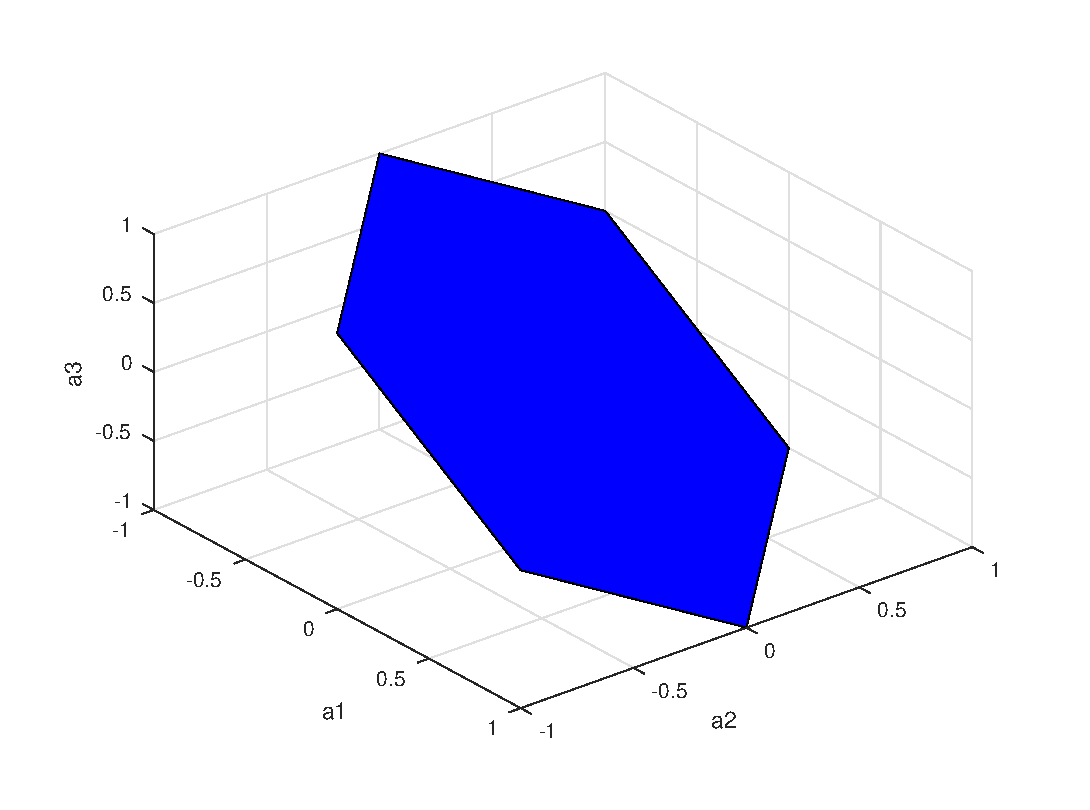
\includegraphics[width=0.5\linewidth]{figPlanoN3_c.eps}
		\end{psfrags}
	\end{center}
	\caption{Feasible region defined by the constraints $-1\leq \dot{\alpha}_i \leq 1$ and $\dot{\alpha}_1+\dot{\alpha}_2+\dot{\alpha}_3=0$. \label{fig:dot:alphas}}

\end{figure}

\lstinputlisting[style=ManualCode]{manual_examples/example_19.m}
For the ordering of $h^1,\ldots,h^6$ in the matrix above, the coefficient
multipliers of $I_2$ are
\[
\begin{array}{c|rrrrrr}
j & 1 & 2 & 3 & 4 & 5 & 6\\ \hline
(1,2,3)h^j & -2 & -1 & 1 & 2 & 1 & -1
\end{array}
\]
The enumerator can permute the columns. Each multiplier applies to every
$\alpha_i\beta_j$, because homogenization multiplies the derivative by
$\sum_i\alpha_i=1$.



\subsubsection*{Example 20}

Suppose that one needs to calculate the derivative of the polynomial \mcode{poly},
defined over two simplexes: the first ($\alpha$) of three vertices, and the second
($\beta$) of two vertices. The variation rates of each parameter are bounded by
\[
 -1 \leq \dot{\alpha}_1(t) \leq 2, \quad -3 \leq \dot{\alpha}_2(t) \leq 4, \quad
 -8 \leq \dot{\alpha}_3(t) \leq 6, \quad
 -4 \leq \dot{\beta}_1(t) \leq 1, \quad -6 \leq \dot{\beta}_2(t) \leq 9.
\]
\lstinputlisting[style=ManualCode]{manual_examples/example_20.m}
On the product of the two simplexes, the diagonal entries of $A$ are
$\alpha_1+3\alpha_2+5\alpha_3+\beta_2$. The derivative is
$(-4\dot\alpha_1-2\dot\alpha_2+\dot\beta_2)I_2$.
The table gives the multiplier of $I_2$ for each pair of rate vertices.
\[
\begin{array}{c|r|rr}
\dot\alpha & -4\dot\alpha_1-2\dot\alpha_2 &
       \dot\beta_2=4 & \dot\beta_2=-1\\ \hline
(-1,-3,4) & 10 & 14 & 9\\
(-1,4,-3) & -4 & 0 & -5\\
(2,-3,1) & -2 & 2 & -3\\
(2,4,-6) & -16 & -12 & -17
\end{array}
\]

If the polynomial is defined from a matrix polynomially dependent on bounded
parameters, then the derivative can be obtained using the syntax

\vspace{0.5cm}%\hspace{2cm}
\noindent\begin{minipage}{\linewidth}
\mcode{>> dotpoly = diff(poly,labelout,bounds,dotbounds)}
\end{minipage}
\vspace{0.2cm}

The rows of \mcode{bounds} contain the parameter intervals. The rows of
\mcode{dotbounds} contain the corresponding lower and upper rate limits.


\subsubsection*{Example 21}

Suppose that one needs to calculate the derivative of the polynomial \mcode{poly},
depending on  parameters $\theta_1$, $\theta_2$ and $\theta_3$. The bounds and
variation rates are given by
\[
 -2 \leq \theta_1(t) \leq 4, \quad
 3 \leq \theta_2(t) \leq 6, \quad
 1 \leq \theta_3(t) \leq 8,
\]
\[
 -1 \leq \dot{\theta}_1(t) \leq 5, \quad
 -3 \leq \dot{\theta}_2(t) \leq 2, \quad
 -7 \leq \dot{\theta}_3(t) \leq 3.
\]

\lstinputlisting[style=ManualCode]{manual_examples/example_21.m}
At $\theta=(1,4,3)$ and $\dot\theta=(5,2,3)$, the chain rule gives
$\dot A=1016I_2$. This value can also be obtained by evaluating the
returned polynomial at the corresponding simplex coordinates.

\subsection*{Command PARTIAL}

The command \mcode{partial} computes the partial derivatives of a polynomial variable with respect
to the simplex parameters. The syntax of \mcode{partial} is

\vspace{0.5cm}%\hspace{2cm}
\noindent\begin{minipage}{\linewidth}
\mcode{>> dpoly = partial(poly,labelout,simpnum)}
\end{minipage}
\vspace{0.2cm}

\noindent where \mcode{poly} is the input polynomial, \mcode{labelout} is the label of the
resulting polynomial, \mcode{simpnum} is the index of the simplex with respect to which the polynomial
is differentiated, and \mcode{dpoly} is a cell structure containing the computed gradient vector.

For instance, suppose that $P(\alpha,\beta)$ is a polynomial with $\alpha$
in a simplex with three vertices, and $\beta$ in a simplex with two vertices. The command

\vspace{0.5cm}%\hspace{2cm}
\noindent\begin{minipage}{\linewidth}
\mcode{>> dpoly = partial(poly,'dPda',1);}
\end{minipage}
\vspace{0.2cm}

\noindent computes the gradient vector
\[
 \frac{\partial P(\alpha,\beta)}{\partial \alpha} =
 \begin{bmatrix}
    \displaystyle \frac{\partial P(\alpha,\beta)}{\partial \alpha_1} & \displaystyle \frac{\partial P(\alpha,\beta)}{\partial \alpha_2} & \displaystyle \frac{\partial P(\alpha,\beta)}{\partial \alpha_3}
 \end{bmatrix}.
\]

Similarly, the command

\vspace{0.5cm}%\hspace{2cm}
\noindent\begin{minipage}{\linewidth}
\mcode{>> dpoly = partial(poly,'dPdb',2);}
\end{minipage}
\vspace{0.2cm}

\noindent yields
\[
 \frac{\partial P(\alpha,\beta)}{\partial \beta} =
 \begin{bmatrix}
    \displaystyle \frac{\partial P(\alpha,\beta)}{\partial \beta_1} & \displaystyle \frac{\partial P(\alpha,\beta)}{\partial \beta_2}
 \end{bmatrix}.
\]

If the variable \mcode{simpnum} is omitted, then the partial derivative is calculated over the first simplex.


\subsubsection*{Example 22}

Consider the polynomial $A(\alpha)$ given by
\[
 A(\alpha) = \alpha_1^2A_1 + \alpha_1\alpha_2A_2 + \alpha_2^2A_3,
\]
defined as the variable \mcode{poly}.
The partial derivative $\displaystyle\frac{\partial A(\alpha)}{\partial \alpha}$ can be computed through the command
\vspace{0.5cm}%\hspace{2cm}
\noindent\begin{minipage}{\linewidth}
\mcode{>> dpoly = partial(poly,'dAda');}
\end{minipage}

The derivatives are taken in the barycentric coordinates before imposing
their unit-sum constraint.
\lstinputlisting[style=ManualCode]{manual_examples/example_22.m}
For the coefficients in the listing, the two cells contain
\[
 \frac{\partial A}{\partial\alpha_1}=(2\alpha_1+3\alpha_2)I_2,\qquad
 \frac{\partial A}{\partial\alpha_2}=(3\alpha_1+10\alpha_2)I_2.
\]


\subsection*{Command DISCSHIFT}

The stability analysis for discrete-time LPV systems can be performed using procedures similar to the ones used in the
continuous-time case. For instance, the discrete-time LPV system
\[
 x(k+1) = A(\alpha(k))x(k), \quad \alpha(k) \in \Delta_N
\]
is asymptotically stable if there exists a symmetric positive definite
matrix $P(\alpha(k))$ satisfying
\[
 A(\alpha(k))'P(\alpha(k+1))A(\alpha(k)) - P(\alpha(k)) < 0.
\]
for all admissible pairs $(\alpha(k),\alpha(k+1))$.

Suppose that $P(\alpha(k))$ is defined as
\[
 P(\alpha(k)) = \sum_{i=1}^N \alpha_i(k) P_i.
\]
Consequently,
\[
 P(\alpha(k+1)) = \sum_{i=1}^N \alpha_i(k+1) P_i.
\]
If the variation rates of the parameters $\alpha(k)$ are bounded, being such bounds previously known and given by
\[
 \underline{d}_i \leq \alpha_i(k+1) - \alpha_i(k) \leq \overline{d}_i, \quad 0 \in [\underline{d}_i, \overline{d}_i], \quad i = 1, \ldots, N,
\]
The admissible pairs form a polytope with vertices
$h^\ell=[(h_0^\ell)' \ (h_1^\ell)']'$, $\ell=1,\ldots,M$.
Both instants use the same $\beta\in\Delta_M$, while
$h_0^\ell,h_1^\ell\in\mathbb R^N$ contain the coordinates at the
current and next instants. For affine $P$,
\[
 \begin{bmatrix}P(\alpha(k))\\ P(\alpha(k+1))\end{bmatrix}
 =\sum_{\ell=1}^{M}\beta_\ell\sum_{i=1}^N
 \begin{bmatrix}h_{0,i}^\ell P_i\\h_{1,i}^\ell P_i\end{bmatrix}.
\]
For $\eta$ steps ahead, each joint vertex has $\eta+1$ blocks,
one for each instant from $k$ to $k+\eta$.


Time-shifted matrices can be automatically computed using the command \mcode{discshift}, whose syntax is

\vspace{0.5cm}%\hspace{2cm}
\noindent\begin{minipage}{\linewidth}
\mcode{>> polyout = discshift(polyin,eta,bounds,targetin,targetout);}
\end{minipage}
\vspace{0.2cm}

The input \mcode{eta} is the number of steps ahead. The rows of
\mcode{bounds} give the lower and upper bounds on each increment.
The inputs \mcode{targetin} and \mcode{targetout} identify the original
simplex and the trajectory simplex, respectively.
If \mcode{bounds} is omitted, the increments may range in $[-1,1]$.
The default \mcode{targetout} is the next available simplex index.
The input \mcode{targetin} can be omitted for a single simplex.
\mcode{discshift} uses MPT3 when available and otherwise tries the
\mcode{cddmex} binary directly. In the absence of both, it supports
one step on a simplex with two vertices using MATLAB alone.
The output has $\eta+1$ cells. Cell $j$ represents the polynomial at
instant $k+j-1$ on the common trajectory simplex.

\subsubsection*{Example 23}

Consider the matrix polynomial $A(\alpha(k))$ given by
\[
 A(\alpha(k)) = \alpha_1(k) \begin{bmatrix} 1 & 0 \\ 0 & 1 \end{bmatrix} + \alpha_2(k) \begin{bmatrix} 3 & 0 \\ 0 & 3 \end{bmatrix},
\]
with
\[
 |\alpha_1(k+1) - \alpha_1(k)| \leq 0.4, \quad  |\alpha_2(k+1) - \alpha_2(k)| \leq 0.6.
\]
The polynomials $A(\alpha(k))$, $A(\alpha(k+1))$ and $A(\alpha(k+2))$, represented in the same simplex domain $\beta \in \Delta_M$,
can be obtained by the command

\vspace{0.5cm}%\hspace{2cm}
\noindent\begin{minipage}{\linewidth}
\mcode{>> polyout = discshift(polyin,2,[-0.4 0.4; -0.6 0.6]);}
\end{minipage}
\vspace{0.2cm}

The output cells \mcode{polyout\{1\}}, \mcode{polyout\{2\}}, and
\mcode{polyout\{3\}} contain $A(\alpha(k))$, $A(\alpha(k+1))$, and
$A(\alpha(k+2))$, respectively.
\lstinputlisting[style=ManualCode]{manual_examples/example_23.m}
There are 14 trajectory vertices. The table pairs the diagonal
coefficients at all three instants. Its rows are sorted by the complete
trajectory values, independently of the enumeration order.
\[
\begin{array}{rrr|rrr}
 k & k+1 & k+2 & k & k+1 & k+2\\ \hline
 1   & 1   & 1   & 2.2 & 3   & 2.2\\
 1   & 1   & 1.8 & 2.2 & 3   & 3\\
 1   & 1.8 & 1   & 2.6 & 1.8 & 1\\
 1   & 1.8 & 2.6 & 3   & 2.2 & 1.4\\
 1.4 & 2.2 & 3   & 3   & 2.2 & 3\\
 1.8 & 1   & 1   & 3   & 3   & 2.2\\
 1.8 & 1   & 1.8 & 3   & 3   & 3
\end{array}
\]



\subsubsection*{Example 24}

Consider now the matrix
\[
 A(\alpha(k),\beta(k)) = \alpha_1(k)\beta_1(k) \begin{bmatrix} 1 & 0 \\ 0 & 1 \end{bmatrix}
 + \alpha_1(k)\beta_2(k) \begin{bmatrix} 3 & 0 \\ 0 & 3 \end{bmatrix}
 + \alpha_2(k)\beta_1(k) \begin{bmatrix} 5 & 0 \\ 0 & 5 \end{bmatrix}
 + \alpha_2(k)\beta_2(k) \begin{bmatrix} 7 & 0 \\ 0 & 7 \end{bmatrix}.
\]

Shift $\alpha$ first and select the cell at $k+1$. Then shift $\beta$
in that polynomial and select the cell at $k+1$ of the second call.
The variable \mcode{shifted} represents $A(\alpha(k+1),\beta(k+1))$.
\lstinputlisting[style=ManualCode]{manual_examples/example_24.m}
A transition from $(\alpha_1(k),\beta_1(k))=(1,1)$ to
$(\alpha_1(k+1),\beta_1(k+1))=(0.6,0.6)$ changes the value
from $I_2$ to $3.4I_2$. At the next instant, the polynomial is
$(7-4\alpha_1(k+1)-2\beta_1(k+1))I_2$.


\subsection*{Command TEXIFY}

The command \mcode{texify}, with syntax given by

\vspace{0.5cm}%\hspace{2cm}
\noindent\begin{minipage}{\linewidth}
\mcode{>> out = texify(poly,option,var1,}$\ldots$\mcode{,varN,simplexnames);}
\end{minipage}
\vspace{0.2cm}

\noindent returns the {\LaTeX} code of the input polynomial \mcode{poly}. The argument
\mcode{option} is a string that specifies whether the desired output format presents an
explicit dependence of the polynomial on the simplexes (\mcode{'explicit'}),
only the polynomial variables without showing their dependence on the simplexes (\mcode{'implicit'}),
or the polynomial structure showing each monomial (\mcode{'polynomial'}). The
arguments \mcode{var1,}$\ldots$\mcode{,varN} are the variables that are used in the expression
to be output; supply each variable separately in such a way that the procedure can
assess the information needed. Finally, the input \mcode{simplexnames} is a cell array of strings
containing the desired names for each simplex, already in {\LaTeX} format. If
only one string is informed instead of a cell array of strings, then it is supposed that
the user intends to represent all the simplexes using one single (multi-simplex) variable.
If \mcode{simplexnames} is omitted, then standard names are used. The name of the
polynomial variables is equal to the \mcode{label} specified in their definition.

\subsubsection*{Example 25}

Let \mcode{Ai} represent $A(\alpha,\beta)$, with degree one and two vertices
in each simplex. Let \mcode{Pi} represent $P(\alpha)$, also of degree one.
In version~3.4, polynomial output requires opcodes. Enable code generation
before creating the variables and the expression. The function below
restores the previous setting on exit.
\lstinputlisting[style=ManualCode]{manual_examples/example_25.m}

The first three fields present the expression as
$A(\alpha,\beta)'P(\alpha)+P(\alpha)A(\alpha,\beta)$,
$A(\alpha)'P(\alpha)+P(\alpha)A(\alpha)$ with grouped parameters, and
$A'P+PA$, respectively. The field \mcode{out.polynomial} contains
the following \LaTeX{} source:
\noindent returns the {\LaTeX} code


\noindent\begin{minipage}{\linewidth}
{\small
\begin{lstlisting}[rulecolor=\color{red}]
out =

\alpha_{1}^{2}\beta_{1}(A_{1}'P_{1}+P_{1}A_{1})
 + \alpha_{1}\alpha_{2}\beta_{1}(A_{1}'P_{2}+A_{2}'P_{1}+P_{1}A_{2}+P_{2}A_{1})
 + \alpha_{2}^{2}\beta_{1}(A_{2}'P_{2}+P_{2}A_{2})
 + \alpha_{1}^{2}\beta_{2}(A_{3}'P_{1}+P_{1}A_{3})
 + \alpha_{1}\alpha_{2}\beta_{2}(A_{3}'P_{2}+A_{4}'P_{1}+P_{1}A_{4}+P_{2}A_{3})
 + \alpha_{2}^{2}\beta_{2}(A_{4}'P_{2}+P_{2}A_{4})
\end{lstlisting}
}
\end{minipage}


\section{Composing matrices and LMIs}\label{construct_lmi}
ROLMIP uses the same matrix and LMI notation as YALMIP.\footnote{Earlier
versions used \mcode{construct\_lmi}. This command remains available for
compatibility.} Consider the parameter-dependent condition
\eqref{eq_estab_discr_param}.
Let \mcode{Ai} and \mcode{Pi} represent $A(\alpha)$ and $P(\alpha)$.
The resulting set of LMIs is constructed by

\vspace{0.5cm}%\hspace{2cm}
\noindent\begin{minipage}{\linewidth}
\mcode{>> LMIs = [[Pi Ai'*Pi; Pi*Ai Pi] >= 0];}
\end{minipage}
\vspace{0.2cm}

ROLMIP performs any necessary degree homogenization.
The MATLAB operators \mcode{>=} and \mcode{<=} specify non-strict
inequalities. To enforce a positive margin, use
\mcode{F >= epsilon*eye(4)} with \mcode{epsilon > 0}, where \mcode{F} is the
$4\times4$ block polynomial. Verify the residual after solving, as described
in Section~\ref{sec_model_diagnostics}.


\subsection{P\'{o}lya's relaxation}\label{subsec_polya}
P\'{o}lya's theorem for homogeneous polynomials with matrix
coefficients~\cite{Sch:03,Sch:05,OP:08b} provides a sufficient condition
for positivity on a product of unit simplexes. Let $F(\alpha)$ denote the
block matrix in \eqref{eq_estab_discr_param}, with all blocks homogenized
to the same degree in each simplex. If $F$ is strictly positive definite
on the product of the simplexes, there are nonnegative integers $d_j$
such that the matrix coefficients of
\begin{equation}\label{eq_cond_estab_discr_polya}
 \left[\prod_{j=1}^M
 \left(\sum_{i=1}^{N_j}\alpha_i^{(j)}\right)^{d_j}\right] F(\alpha)
\end{equation}
are positive definite. Each factor equals one on its simplex.

ROLMIP implements P\'{o}lya's relaxation through \mcode{polya}:

\vspace{0.5cm}%\hspace{2cm}
\noindent\begin{minipage}{\linewidth}
	\mcode{>> polyout = polya(polyin,d);}
\end{minipage}
\vspace{0.2cm}

The vector \mcode{d} specifies the degree increase for each simplex.
A scalar \mcode{d} in a multi-simplex model applies only to the first
simplex. Omitting the second argument applies degree one to each simplex.

\subsubsection*{Example 26}

The implementation of the LMIs resulting from the matrix polynomial~\eqref{eq_cond_estab_discr_polya} being
positive definite can be performed through the following sequence of commands.

\begin{minipage}{11.5cm}
 \begin{lstlisting}
%Example 26
A{1} = {[1 0],eye(2)};
A{2} = {[0 1],2*eye(2)};

polyA = rolmipvar(A,'A',2,1);
polyP = rolmipvar(2,2,'P','sym',2,1);
cond = [polyP polyA'*polyP; polyP*polyA polyP];
LMIs = [cond >= 0]
d = 3;
condpolya = polya(cond,d);
LMIspolya = [condpolya >= 0]
 \end{lstlisting}
\end{minipage}
\vspace{0.2cm}

\begin{minipage}{9.2cm}
\begin{lstlisting}[rulecolor=\color{red}]
>> LMIs
++++++++++++++++++++++++++++++++
|   ID|              Constraint|
++++++++++++++++++++++++++++++++
|   #1|   Matrix inequality 4x4|
|   #2|   Matrix inequality 4x4|
|   #3|   Matrix inequality 4x4|
++++++++++++++++++++++++++++++++


>> LMIspolya
++++++++++++++++++++++++++++++++
|   ID|              Constraint|
++++++++++++++++++++++++++++++++
|   #1|   Matrix inequality 4x4|
|   #2|   Matrix inequality 4x4|
|   #3|   Matrix inequality 4x4|
|   #4|   Matrix inequality 4x4|
|   #5|   Matrix inequality 4x4|
|   #6|   Matrix inequality 4x4|
++++++++++++++++++++++++++++++++
\end{lstlisting}
\end{minipage}
\vspace{0.2cm}
\vspace{0.2cm}

Note the increased number of LMIs after the application of P\'{o}lya's relaxation.

% \begin{minipage}{9.2cm}
% \begin{lstlisting}[rulecolor=\color{red}]
%
% \end{lstlisting}
% \end{minipage}

In the following section, more involved examples based on uncertain linear systems problems are presented for a better understanding of ROLMIP.

\section{Solving Uncertain Linear Systems Problems with ROLMIP}

\subsection{Robust Stability Analysis}

Consider the problem of robust stability analysis of the discrete-time linear system given in \eqref{eq_discr_system} with the following uncertain dynamic matrix
\[
A(\alpha)=\alpha_1\begin{bmatrix}0.1 & 0.9 \\0 & 0.1 \end{bmatrix} + \alpha_2\begin{bmatrix}0.5 & 0 \\1 & 0.5 \end{bmatrix}
\]
The first step is the the declaration of $A(\alpha)$ as a \mcode{rolmipvar}, which can be performed as (there are other possibilities)

\vspace{0.5cm}%\hspace{2cm}
\begin{minipage}{8.5cm}
	\mcode{>> A\{1\} = [0.1 0.9;0 0.1];}\\
	\mcode{>> A\{2\} = [0.5 0;1 0.5];}\\
	\mcode{>> A = rolmipvar(A,'A(}\textbackslash\mcode{alpha)',2,1)}
\end{minipage}
\vspace{0.2cm}

\noindent and the last command prints in screen:

\begin{minipage}{11.2cm}
	\begin{lstlisting}[rulecolor=\color{red}]
		Label: A(\alpha)
		Vertices: [2]
		Degrees:  [1]

		a1*[0.1         0.9]  + a2*[0.5           0]
		[0         0.1]         [1         0.5]
	\end{lstlisting}
\end{minipage}

The next step is to choose the structure for the Lyapunov matrix. For instance, consider an affine (degree one) polynomial dependence on $\alpha$, as in \eqref{eq_aalfa_politopico}. In this case the declaration of $P(\alpha)$ is done through the command

\vspace{0.5cm}%\hspace{2cm}
\begin{minipage}{8.5cm}
	\mcode{>> P = rolmipvar(2,2,'P(}\textbackslash\mcode{alpha)',2,1)}\\
\end{minipage}
\vspace{0.2cm}

\noindent echoing in screen

\begin{minipage}{13.5cm}
	\begin{lstlisting}[rulecolor=\color{red}]
		Linear matrix variable 2x2 (symmetric, real, 3 variables)
		Label: P(\alpha)
		Vertices: [2]
		Degrees:  [1]
	\end{lstlisting}
\end{minipage}

As shown in last section, the programming of the robust stability condition is very easy (the echo in screen, produced by YALMIP, is also shown):

\vspace{0.5cm}
\begin{minipage}{20.5cm}
	\mcode{>> LMIs = [[P A'*P; P*A P] >= 0]}
\end{minipage}

\begin{minipage}{9.2cm}
	\begin{lstlisting}[rulecolor=\color{red}]
		++++++++++++++++++++++++++++++++
		|   ID|              Constraint|
		++++++++++++++++++++++++++++++++
		|   #1|   Matrix inequality 4x4|
		|   #2|   Matrix inequality 4x4|
		|   #3|   Matrix inequality 4x4|
		++++++++++++++++++++++++++++++++
	\end{lstlisting}
\end{minipage}


Note that the number of LMIs (three) agrees with the number of monomials  of the expression given in \eqref{eq_poly_lmi} when $N=2$. Actually, each monomial gives rise to one LMI. After solving the set of LMIs (using SeDuMi) with the command:

\vspace{0.5cm}
\begin{minipage}{20.5cm}
	\mcode{>> optimize(LMIs,[],sdpsettings('verbose',0,'solver','sedumi'));} %TROQUEI POIS O SOLVESDP ESTA OBSOLETO, SEGUNDO O YALMIP
\end{minipage}
\vspace{0.2cm}

\noindent and checking the status of the constraints after the optimization, one has

\begin{minipage}{15.0cm}
	\begin{lstlisting}[rulecolor=\color{red}]
		>> checkset(LMIs)

		++++++++++++++++++++++++++++++++++++++++++++++++++++++++++++++++
		|   ID|          Constraint|   Primal residual|   Dual residual|
		++++++++++++++++++++++++++++++++++++++++++++++++++++++++++++++++
		|   #1|   Matrix inequality|           0.17957|      1.9148e-14|
		|   #2|   Matrix inequality|           0.12168|       3.058e-14|
		|   #3|   Matrix inequality|          0.056108|      2.2844e-14|
		++++++++++++++++++++++++++++++++++++++++++++++++++++++++++++++++
	\end{lstlisting}
\end{minipage}

As the primal residuals are positive, the LMIs are strictly feasible, assuring the robust stability of $A(\alpha)$. Moreover, the Lyapunov matrix that certifies the robust stability can be inspected using the command:

\begin{minipage}{15.0cm}
	\begin{lstlisting}[rulecolor=\color{red}]
		>> double(P)
		Label: P(\alpha)
		Vertices: [2]
		Degrees:  [1]

		a1*[0.56664   0.0039574]    + a2*[1.0987    0.062489]
		[0.0039574     0.87634]       [0.062489     0.45827]
	\end{lstlisting}
\end{minipage}

It is worth to emphasize that, depending on the solver used or on the MATLAB version, different values for $P(\alpha)$ can be obtained.
A script with the implementation of the present section can be found into the folder \texttt{manual\_examples}, with the name
\texttt{example\_Section\_7\_1.m}.

\subsection{Guaranteed $\Hi$ Cost Computation}\label{sec_example}

Consider the continuous-time uncertain time-invariant system
given by
\begin{equation}\label{eq_syst}
\left\{\begin{array}{rl}
\dot{x}(t) = & A(\alpha)x(t) + B(\alpha)w(t)\\
y(t) = & C(\alpha)x(t) + D(\alpha)w(t)
\end{array}\right.
\end{equation}
with $A(\alpha) \in \mathbb{R}^{n \times n}$, $B(\alpha) \in \mathbb{R}^{n \times r}$,
$C(\alpha) \in \mathbb{R}^{q \times n}$ and $D(\alpha) \in \mathbb{R}^{q \times r}$.
The transfer function from the disturbance input $w$ to the output $y$, for a fixed $\alpha$,
is given by
\[
 H(s,\alpha) = C(\alpha) \big( s \mbox{I} - A(\alpha) \big)^{-1} B(\alpha) + D(\alpha)
\]
The bounded real lemma assures the Hurwitz stability of $A(\alpha)$
(\textit{i.e.}, all eigenvalues have negative real part)
for all $\alpha \in \Delta_N$ and an upper bound $\gamma$ on the $\Hi$ norm of the transfer
function from $w$ to $y$. It can be formulated as follows \cite{BEFB:94}.

\begin{Plema}
Matrix $A(\alpha)$ is Hurwitz and $\| H(s,\alpha) \|_{\infty} < \gamma$ for all $\alpha \in \Delta_N$
if there exists a symmetric positive definite matrix $P(\alpha) = P(\alpha)' > 0$
such that
\begin{equation}\label{eq_cond_hinf}
\left[ \begin{matrix}
A(\alpha)'P(\alpha) + P(\alpha)A(\alpha) + C(\alpha)'C(\alpha) &  \star\\
B(\alpha)'P(\alpha) + D(\alpha)'C(\alpha) & D(\alpha)'D(\alpha) - \gamma^2\mathbf{I}
\end{matrix}  \right]
  < 0 ,  ~~~~\forall \alpha \in \Delta_N
\end{equation}
\end{Plema}

In this example, consider a fourth-order mass-spring system, also investigated
in \cite{OP:08b}, whose matrices are given by
\begin{align*}
 A = \begin{bmatrix}
      0 & 0 & 1 & 0 \\
      0 & 0 & 0 & 1 \\
      -\frac{2}{m_1} & \frac{1}{m_1} & -\frac{c_0}{m_1} & 0 \\
      \frac{1}{m_2} & -\frac{1}{m_2} & 0 & -\frac{c_0}{m_2}
     \end{bmatrix}, \quad
 B = \begin{bmatrix} 0 \\ 0 \\ \frac{1}{m_1} \\ 0 \end{bmatrix}, \quad
 C = \begin{bmatrix} 0 & 1 & 0 & 0 \end{bmatrix}, \quad D = 0,
\end{align*}
with
\[
 0.5 \leq m_1 \leq 1.5, \quad 0.75 \leq m_2 \leq 1.25, \quad 1 \leq c_0 \leq 3.
\]

Setting $\theta_1 = 1/m_1$, $\theta_2 = 1/m_2$ and $\theta_3 = c_0$, one has
\[
 2/3 \leq \theta_1 \leq 2, \quad 0.8 \leq \theta_2 \leq 4/3, \quad 1 \leq \theta_3 \leq 3,
\]
and the matrices can be rewritten as
\begin{align*}
 A(\theta) &=
 \begin{bmatrix} 0 & 0 & 1 & 0 \\ 0 & 0 & 0 & 1 \\ 0 & 0 & 0 & 0 \\ 0 & 0 & 0 & 0 \end{bmatrix}
 + \theta_1 \begin{bmatrix} 0 & 0 & 0 & 0 \\ 0 & 0 & 0 & 0 \\ -2 & 1 & 0 & 0 \\ 0 & 0 & 0 & 0 \end{bmatrix}
 + \theta_1\theta_3 \begin{bmatrix} 0 & 0 & 0 & 0 \\ 0 & 0 & 0 & 0 \\ 0 & 0 & -1 & 0 \\ 0 & 0 & 0 & 0 \end{bmatrix}\\
 &\quad + \theta_2 \begin{bmatrix} 0 & 0 & 0 & 0 \\ 0 & 0 & 0 & 0 \\ 0 & 0 & 0 & 0 \\ 1 & -1 & 0 & 0 \end{bmatrix}
 + \theta_2\theta_3 \begin{bmatrix} 0 & 0 & 0 & 0 \\ 0 & 0 & 0 & 0 \\ 0 & 0 & 0 & 0 \\ 0 & 0 & 0 & -1 \end{bmatrix},\\
 B(\theta) &= \theta_1 \begin{bmatrix} 0 \\ 0 \\ 1 \\ 0 \end{bmatrix}, \quad
 C(\theta) = \begin{bmatrix} 0 & 1 & 0 & 0 \end{bmatrix}, \quad D(\theta) = 0.
\end{align*}

The following algorithm minimizes $\mu=\gamma^2$ subject to the
coefficient LMIs. The listing is read directly from
\texttt{Algorithm\_1\_Section\_6.m}.
The polynomial $B(\theta)$ uses a single exponent and a single interval
because it depends only on $\theta_1$. The matrix $T$ is replaced by
its P\'{o}lya expansion before the coefficient constraints are assembled.
The code checks the solver status and the constraint residuals before
returning $\sqrt{\mu}$.
\noindent\begin{minipage}{\linewidth}
\begin{algorithm}\label{algo_hinf}
\lstinputlisting[numbers=left,xleftmargin=2em,style=ManualCode]{manual_examples/Algorithm_1_Section_6.m}
\end{algorithm}
\end{minipage}


\begin{remark}\label{rem_issues}
The expression for \mcode{T22} combines the \mcode{rolmipvar} \mcode{Di}
with the \mcode{sdpvar} \mcode{mu}. Because the \mcode{rolmipvar} expression
is on the left, its class handles the subtraction. The reverse order may
dispatch the operation to YALMIP.
\end{remark}


Changing \mcode{degP} changes the degree of the Lyapunov polynomial
and hence the set of sufficient LMIs. Table~\ref{tab_results_hinf} reports
the bounds obtained with \mcode{d = [0 0 0]}.
With degree two, the reported bound agrees to the displayed precision
with the worst-case reference of $1.0108$.

\begin{table}[!ht]
\caption{Values of $\gamma^{\ast}= \min \gamma$ obtained when varying the degree of the
polynomial variable~$P(\alpha)$.}\label{tab_results_hinf}
\begin{center}
\begin{tabular}{A|A} \hline \hline
 \mcode{degP} & $\gamma^{\ast}$ \\
\hline 0 & 2.8429 \\
\hline 1 & 1.0540 \\
\hline 2 & 1.0108 \\
\hline 3 & 1.0108 \\
\hline 4 & 1.0108 \\
\hline 5 & 1.0108 \\ \hline
\end{tabular}
\end{center}
\end{table}

To reproduce the P\'{o}lya relaxation in Algorithm~\ref{algo_hinf}, pass
\mcode{d = [3 3 3]} to increase the degree on each of the three simplexes.
The relaxation is applied to \mcode{T} before constructing \mcode{LMIs}.
A scalar \mcode{d = 3} would relax only the first simplex.

Table~\ref{tab_results_hinf_polya} reports the resulting bounds.

\begin{table}[!ht]
\caption{Values of $\gamma^{\ast}= \min \gamma$ obtained when varying the degree of the
polynomial variable~$P(\alpha)$ for $d = 3$.}\label{tab_results_hinf_polya}
\begin{center}
\begin{tabular}{A|A} \hline \hline
 \mcode{degP} & $\gamma^{\ast}$ \\
\hline 0 & 2.8429 \\
\hline 1 & 1.0308 \\
\hline 2 & 1.0108 \\
\hline 3 & 1.0108 \\
\hline 4 & 1.0108 \\
\hline 5 & 1.0108 \\ \hline
\end{tabular}
\end{center}
\end{table}


% \section{Creating a MATLAB executable file}\label{sec_lmifiles}
% Although the Robust LMI Parser toolbox is a very practical package and allows
% the programming of complex parameter-dependent LMIs without
% spending much effort, it is true that
% the computational time required for the toolbox to compose the LMIs is considerably
% higher than setting the LMIs monomial by monomial. To circumvent this drawback
% it is possible to use the Robust LMI Parser to create a MATLAB executable file
% that solves the same set of LMIs without consuming much time.
% To do so it is necessary to use the command \texttt{lmifiles} to open the file,
% to insert the LMIs and to close the file.
%
% The syntax used for opening the file is
% \[
% \mbox{\tt fid = lmifiles('open',filename)}.
% \]
% The first argument may be replaced by \texttt{'o'}. The parameter \texttt{filename}
% is both the name of the file and the name of the main function, being
% declared without the extension \texttt{.m}. The file identifier \texttt{fid} associated
% is returned. The file must be opened at least before the definition of the first LMI, but
% it is recommended to open the file before the definition of the first variable.
%
%
% The insertion of the informations on the problem to be solved are done by using the
% \texttt{lmifiles} procedure in either of the following syntaxes.
% \begin{itemize}
% \item To insert an LMI:
% \[
% \mbox{\tt lmifiles('insert',fid,Term,ineq)}.
% \]
% The first argument may be replaced by \texttt{'i'}. The parameter \texttt{fid} is the
% file identifier returned when opening the file. The structure \texttt{Term} is the cell
% array that defines the LMI, in which \texttt{Term\{i,j\}} corresponds to the
% element $(i,j)$ of the matrix, and \texttt{ineq} is the signal of the inequality.
%
% \item To define the objective function:
% \[
% \mbox{\tt lmifiles('insert',fid,obj\_min)}.
% \]
% The parameter \texttt{obj\_min} is the label of the variable to be minimized.
%
% \item To define the settings of the optimization procedure:
% \[
% \mbox{\tt lmifiles('insert',fid,'sdpsettings','name1','value1','name2','value2',...)}.
% \]
% The argument \texttt{'sdpsettings'} is used to specify that the following arguments will be
% the names and values of the properties of the solver options to be changed. The options names
% and values are the ones used in the command \texttt{solvesdp} of the YALMIP toolbox \cite{Lof:04}.
% \end{itemize}
%
%
% After inserting all the informations of the problem, the file needs to be closed by using the command
% \[
% \mbox{\tt lmifiles('close',fid)}.
% \]
% The first argument may be replaced by \texttt{'c'}. The new MATLAB executable
% file is stored at the same directory of the program used to create it. The input
% parameters of the main function are the system matrices and other user-defined
% variables, and the output is a structure whose fields contain the values of the
% resulting variables, if the LMI could be solved.
%
% \subsection*{Example 10}
% The creation of a MATLAB executable file to solve the LMI presented in
% \eqref{eq_estab_discr_param}, considering a system with $N = 2$ vertices and polynomial variables with
% degree $g = 1$, can be done through the following sequence of MATLAB commands
%
% \vspace{0.5cm}%\hspace{2cm}
% \begin{minipage}{8.5cm}
% {\tt >> fid = lmifiles('o','discr\_stab');} \\
% {\tt >> poly\_struct(A,'A',2,1);} \\
% {\tt >> poly\_struct(P,'P',2,1);} \\
% {\tt >> Term\{1,1\} = parser\_poly('P');}\\
% {\tt >> Term\{1,2\} = parser\_poly('A''*P');}\\
% {\tt >> Term\{2,2\} = parser\_poly('P');}\\
% {\tt >> lmifiles('i',fid,Term,'>');} \\
% {\tt >> lmifiles('c',fid);}
% \end{minipage}
% \vspace{0.2cm}
%
% The resulting function can then be called through the command
%
% \vspace{0.5cm}%\hspace{2cm}
% \begin{minipage}{8.5cm}
% {\tt >> Output = discr\_stab(A);}
% \end{minipage}
% \vspace{0.2cm}


\section{Model Diagnostics and Solution Verification}\label{sec_model_diagnostics}
The commands in this section are available in ROLMIP~3.4. They can be
used to measure the construction of an LMI model, inspect its formulation,
and check the numerical values returned after solving it.

\subsection*{Commands ROLMIP\_BEGIN and ROLMIP\_END}
Call \mcode{rolmip\_begin} before declaring the decision variables and
constructing the LMIs. Stop the timer before calling the solver.
\begin{lstlisting}
rolmip_begin;
% Define the variables and construct LMIs.
[time,V,L] = rolmip_end(LMIs);
\end{lstlisting}
The output \mcode{time} is the elapsed wall time in seconds, including
polynomial operations and any other work in the timed interval. The timer
stops before the statistics are computed. The output \mcode{V} is the
number of distinct scalar decision variables that appear in \mcode{LMIs}.
The output \mcode{L} is the sum of the orders of the blocks classified by
YALMIP as semidefinite constraints. Elementwise inequalities and equalities
do not contribute to \mcode{L}. Call \mcode{rolmip\_begin} again for a new
measurement.

\subsection*{Command ROLMIP\_CHECK}
The command \mcode{rolmip\_check} inspects a matrix polynomial. It checks
the dimensions and exponent vectors, the homogeneity on each simplex, and
whether the coefficients are finite, real, symmetric, and affine in the
decision variables. To check whether the expression is suitable for an LMI,
use
\begin{lstlisting}
report = rolmip_check(poly,'lmi',true);
report.lmi_ready
report.issues
\end{lstlisting}
The field \mcode{issues} gives the severity and location of each problem.
Use \mcode{rolmip\_check(poly)} to inspect intermediate expressions, which
can be rectangular or nonsymmetric. Affinity here refers to the decision
variables. A polynomial of degree greater than one in the uncertain
parameters can still define an LMI.

\subsection*{Diagnostic session commands}
To inspect the ROLMIP inequalities as they are constructed, start a
diagnostic session:
\begin{lstlisting}
rolmip_check_begin;
% Construct the ROLMIP inequalities.
partial = rolmip_check_report;
report = rolmip_check_end;
\end{lstlisting}
The command \mcode{rolmip\_check\_report} reads the report during the session.
The command \mcode{rolmip\_check\_end} stops the collection and returns the
final report. Repeated issues within one condition are grouped, with the
source file and line recorded when available. Check
\mcode{report.has\_errors} and \mcode{report.has\_warnings} before calling the
solver. This session observes the ROLMIP inequalities at construction time.
Constraints written directly in YALMIP can be inspected after solving by
passing the final set to \mcode{rolmip\_verify}.

\subsection*{Command ROLMIP\_LMI}
Use \mcode{rolmip\_lmi} when the relation between the coefficient
constraints and the monomials of a particular inequality is needed.
\begin{lstlisting}
[F,origin] = rolmip_lmi(poly,'>=','Positivity');
\end{lstlisting}
Here \mcode{poly} is the complete residual polynomial. For a comparison
between two polynomials, form their difference first. The relation can be
\mcode{'>='} or \mcode{'<='}. The command requires real, symmetric
coefficients that are affine in the decision variables. If a P\'{o}lya
relaxation is desired, apply \mcode{polya} to the residual before this call.
The structure \mcode{origin} records the signed coefficient matrices,
their exponents, and their indices local to \mcode{F}.

\subsubsection*{Example 27}
On a two-vertex simplex, let $X$ be a symmetric $2\times 2$ decision
matrix and define
\[
  P(\alpha)=\alpha_1^2 X+\alpha_1\alpha_2 I_2+\alpha_2^2(X+I_2).
\]
The following commands construct coefficient constraints for
$P(\alpha)\succeq 0$ and display the index in \mcode{F} associated with
each monomial.

\lstinputlisting[style=ManualCode]{manual_examples/example_27.m}

The monomials $\alpha_1^2$ and $\alpha_2^2$ correspond to
\mcode{F(1)} and \mcode{F(2)}, respectively. The index for
$\alpha_1\alpha_2$ is empty because its coefficient $I_2$ is
constant and positive definite.

\subsection*{Command ROLMIP\_VERIFY}
After solving the model, call \mcode{rolmip\_verify} with the complete
YALMIP constraint set:
\begin{lstlisting}
solution = optimize(LMIs,[],options);
report = rolmip_verify(LMIs,'solver',solution);
\end{lstlisting}
This command checks real semidefinite blocks, elementwise inequalities,
and equalities at the current values of the decision variables. The fields
\mcode{violated\_indices} and \mcode{unevaluable\_indices} locate violated
constraints and constraints that could not be checked. The field
The field \mcode{constraints\_passed} summarizes numerical feasibility
for the current values. The report records the solver status separately.
The arguments \mcode{'abs\_tol'} and \mcode{'rel\_tol'} set the absolute
and relative tolerances. Both default to $10^{-8}$.

To inspect an individual polynomial inequality, pass the \mcode{origin}
returned by \mcode{rolmip\_lmi}. The optional \mcode{'points'} argument
evaluates the signed polynomial at selected parameter values, with one
barycentric row per simplex in each point. For a two-vertex simplex:
\begin{lstlisting}
points = {{[1 0]}, {[0.5 0.5]}, {[0 1]}};
report = rolmip_verify(origin,'solver',solution,'points',points);
\end{lstlisting}
The field \mcode{certificate\_passed} reports the coefficient check
within the numerical tolerances. The field \mcode{samples\_passed}
reports the point check. Mathematically, positive semidefiniteness
of every signed coefficient is sufficient over the entire multi-simplex.
A successful sample check applies only to the selected points.
Evaluating these points requires \mcode{origin}, which retains
the monomial exponents.

\subsubsection*{Example 28}
Consider a continuous-time system with two vertices and fixed uncertain
parameters. The following commands construct a Lyapunov condition,
measure the model construction, and check the solution. The origin of the
Lyapunov inequality is saved so that it can also be evaluated at the
midpoint of the simplex.
\lstinputlisting[style=ManualCode]{manual_examples/example_28.m}
The measured time includes the work of the diagnostic session.
In the tested MATLAB environment, the model had $V=6$ scalar variables
and $L=10$ semidefinite rows. The three checks passed. The session report
covers the conditions constructed during the session, including those
discarded later. The call with \mcode{LMIs} checks the final set of
constraints. To measure construction alone, time the model with the
diagnostic session disabled.

\section{Utilities}\label{sec_utilities}

\subsection*{Command ROLMIP\_VOLUME}
The command \mcode{rolmip\_volume} measures the region
\[
  \mathcal E(P) = \{x \in \mathbb R^n : x^\top P(\alpha)x \le 1
                      \text{ for all } \alpha \in \Delta_N\}.
\]
For a constant $P$, the region
is a single ellipsoid. For affine dependence,
$P(\alpha)=\sum_{i=1}^{N}\alpha_iP_i$, the region is the intersection of
the $N$ vertex ellipsoids.

\begin{lstlisting}[style=ManualCode]
[V,info] = rolmip_volume(P);
[V,info] = rolmip_volume(P,'subspace',[1 3],'reduction','cut');
\end{lstlisting}

Pass a numeric matrix, a cell array of vertex matrices, or a
\mcode{rolmipvar} with numeric coefficients on one simplex.
For a matrix obtained through from an LMI-based condition, pass \mcode{value(P)} after solving.
The matrix $P(\alpha)$ must be symmetric and positive definite
throughout the simplex. The full region and coordinate cuts also
support polynomial dependence of any degree on a two-vertex simplex.

The optional argument \mcode{'subspace'} selects the coordinates to keep
and defaults to all $n$ coordinates. The default reduction,
\mcode{'projection'}, allows the omitted coordinates to vary. For each
projected point, a single choice of those coordinates must satisfy all
vertex inequalities. A projection of an affine intersection onto fewer
coordinates uses YALMIP and a conic solver, selectable with
\mcode{'Solver'}. The \mcode{'cut'} reduction sets the omitted
coordinates to zero.

For constant $P$, the measure follows from a closed-form formula.
For intersections, the command measures interval length in 1D,
estimates area by angular quadrature in 2D, and estimates volumes by
spherical Monte Carlo in higher dimensions. The option
\mcode{'NumDirections'} controls the number of
directions, and \mcode{info.standardError} reports the sampling standard
error of the Monte Carlo estimate.

Use \mcode{'plot',1} to draw the result in 2D or 3D. Plotting is off
by default. Set \mcode{'color'} to a MATLAB color name or an RGB triplet.
The option \mcode{'FaceAlpha'} controls surface opacity in 3D.
For a 2D plot with multiple vertices, \mcode{'drawVertices',1} adds the
dotted vertex contours. The columns of \mcode{info.boundaryX} give the
sampled boundary points in the selected coordinates. In 2D,
\mcode{info.contour} repeats the first point at the end so it can be
plotted directly as a closed curve, even with plotting disabled.

\pagebreak
\subsubsection*{Example 29}
The following commands compute the area of the intersection of three
ellipses. The second and third ellipses are rotations of the first by
$60^\circ$ and $120^\circ$, respectively. Figure~\ref{fig_volume_2d}
shows the sampled boundary and the three vertex contours.

\lstinputlisting[style=ManualCode]{manual_examples/example_29.m}

The exact area is $3\arctan(1/(2\sqrt{3}))$. MATLAB returns $0.8431$,
which agrees to four decimal places.

\begin{figure}[!htb]
  \centering
  \begin{psfrags}
    \psfrag{x1}[c][c]{$x_1$}
    \psfrag{x2}[c][c][1][-90]{$x_2$}
  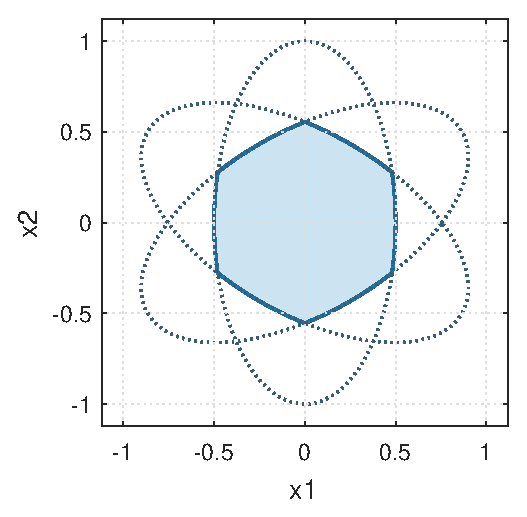
\includegraphics[width=0.50\linewidth]{rolmip-volume-2d.eps}
  \caption{Intersection in Example 29 (shaded).
        The dotted curves are the three vertex ellipses.\label{fig_volume_2d}	 }
  \end{psfrags}
\end{figure}

\section{Conclusion}\label{sec_conclusion}
The Robust LMI Parser automates the construction of sufficient LMIs from
parameter-dependent matrix inequalities. Its polynomial operations apply
to homogeneous polynomials of arbitrary degree on unit simplexes or to
polynomials in parameters with known intervals. Suggestions for improvement
and bug reports are welcome at \texttt{agulhari@utfpr.edu.br}.


% Ack - foi colocado como footnote na primeira pagina
% \begin{ack}
%  This work was supported by CNPq, CAPES and FAPESP.
% \end{ack}
%





\clearpage
\appendix
\section{Version history}\label{app_version_history}

The entries below summarize the
\href{https://github.com/rolmip/rolmip/releases}{GitHub releases}.
Where the release notes give only a general description, the entry
summarizes the changes between the adjacent tags.

\subsection*{Tagged releases}

\begin{description}
\setlength{\itemsep}{2pt}
\item[\href{https://github.com/rolmip/rolmip/releases/tag/1.0}{1.0}]
  First tagged release. It introduced \texttt{poly\_struct} to define
  polynomial matrices and \texttt{parser\_poly} to parse expressions.
  The toolbox also constructed coefficient LMIs and used
  \texttt{lmifiles} to generate reusable MATLAB files.
\item[\href{https://github.com/rolmip/rolmip/releases/tag/1.1}{1.1}]
  Added syntax for assigning each coefficient matrix to a monomial
  by specifying its exponent vector.
\item[\href{https://github.com/rolmip/rolmip/releases/tag/2.0}{2.0}]
  Introduced products of separate unit simplexes and added
  \texttt{affine2poly} to convert affine parameter dependence to this
  representation.
\item[\href{https://github.com/rolmip/rolmip/releases/tag/2.1}{2.1}]
  Simplified the declaration of constant matrices and adapted LMI
  construction to the YALMIP interface used at the time.
  Added \texttt{poly\_derive} for time derivatives with bounded rates.
\item[\href{https://github.com/rolmip/rolmip/releases/tag/2.2}{2.2}]
  Restored \texttt{product\_poly} for polynomial multiplication.
  Revised the derivative calculation and homogenization across rate
  simplexes. See the
  \href{https://github.com/rolmip/rolmip/compare/2.1...2.2}{code comparison}.
\item[\href{https://github.com/rolmip/rolmip/releases/tag/2.3}{2.3}]
  Revised monomial indexing to use per-simplex exponent tables in
  several routines. Improved vertex-count checks during parsing and LMI
  assembly, and corrected the single-simplex case in \texttt{poly\_derive}.
  See the \href{https://github.com/rolmip/rolmip/compare/2.2...2.3}{code comparison}.
\item[\href{https://github.com/rolmip/rolmip/releases/tag/3.0a}{3.0a}]
  Introduced \texttt{rolmipvar}, with MATLAB operators for polynomial
  arithmetic, matrix assembly, and inequalities. Added methods for
  parameter evaluation, derivatives, discrete-time shifts, and \LaTeX{}
  generation, together with manual examples.
\item[\href{https://github.com/rolmip/rolmip/releases/tag/3.0}{3.0}]
  Updated the manual and its examples. Added \texttt{coeffs} for retrieving
  coefficients and exponents and preserved parameter bounds in polynomial
  arithmetic. See the
  \href{https://github.com/rolmip/rolmip/compare/3.0a...3.0}{code comparison}.
\item[\href{https://github.com/rolmip/rolmip/releases/tag/3.1}{3.1}]
  Added Octave compatibility changes, including dimension handling
  through \texttt{size} and \texttt{ndims}. Also corrected matrix
  exponentiation and revised coefficient counting in the constructor.
\item[\href{https://github.com/rolmip/rolmip/releases/tag/3.2}{3.2}]
  Added coefficient-wise \texttt{round}. The constructor now inserts a
  simplex for a bounded parameter that does not occur explicitly in the
  polynomial. See the
  \href{https://github.com/rolmip/rolmip/compare/3.1...3.2}{code comparison}.
\item[\href{https://github.com/rolmip/rolmip/releases/tag/3.3}{3.3}]
  Updated \texttt{diff} to check that the rate intervals contain zero
  and to handle fixed parameter bounds when converting rates to simplex
  coordinates.
\end{description}

\subsection*{3.4}

The current version includes optimized polynomial operations, bounded caches, corrections
to polynomial and LMI construction, and parser timing with model size
statistics. The draft also consolidates the coefficient and exponent
accessors. As new features, one has the model diagnostics and solution verification in
Section~\ref{sec_model_diagnostics}, the pruned internal rate enumeration
in \texttt{diff}, and the additional vertex enumeration paths in
\texttt{discshift}, and the quadratic region volume utility in
Section~\ref{sec_utilities}.


\clearpage
%\bibliographystyle{IEEEtran}
\bibliographystyle{plain}

%\bibliography{listacompleta,newlistacompleta,estgeral,hinf,filtering,hoofilt,robust,fldp,saida,switched,estquad,markov,sdp,fuzzy,fragile,satcon,estab,ltv,polinomial,scheduling,bmi,ncs,mpc,delay,sispot,cristiano_new,newbib,newbib_cristiano}

\begin{thebibliography}{10}

\bibitem{AA:00}
E.~D. Andersen and K.~D. Andersen.
\newblock The {MOSEK} interior point optimizer for linear programming: An
  implementation of the homogeneous algorithm.
\newblock In H.~Frenk, K.~Roos, T.~Terlaky, and S.~Zhang, editors, {\em High
  Performance Optimization}, volume~33 of {\em Applied Optimization}, pages
  197--232. Springer US, 2000.
\newblock \url{http://www.mosek.com}.

\bibitem{AF:92}
D.~Avis and K.~Fukuda.
\newblock A pivoting algorithm for convex hulls and vertex enumeration of
  arrangements and polyhedra.
\newblock {\em Discrete \& Computational Geometry}, 8(3):295--313, September
  1992.

\bibitem{BOMP:06b}
P.-A. Bliman, R.~C. L.~F. Oliveira, V.~F. Montagner, and P.~L.~D. Peres.
\newblock Existence of homogeneous polynomial solutions for parameter-dependent
  linear matrix inequalities with parameters in the simplex.
\newblock In {\em Proceedings of the 45th IEEE Conference on Decision and
  Control}, pages 1486--1491, San Diego, CA, USA, December 2006.

\bibitem{BEFB:94}
S.~Boyd, L.~{El Ghaoui}, E.~Feron, and V.~Balakrishnan.
\newblock {\em Linear Matrix Inequalities in System and Control Theory}.
\newblock SIAM Studies in Applied Mathematics, Philadelphia, PA, 1994.

\bibitem{rromulocconf}
M.~Chamanbaz, F.~Dabbene, D.~Peaucelle, and R.~Tempo.
\newblock {R-RoMulOC}: {A} unified tool for randomized and robust
  multiobjective control.
\newblock In {\em Proceedings of the 8th IFAC Symposium on Robust Control
  Design (ROCOND 2015)}, volume~48, pages 144--149, Bratislava, July 2015.

\bibitem{CGTV:07}
G.~Chesi, A.~Garulli, A.~Tesi, and A.~Vicino.
\newblock Robust stability of time-varying polytopic systems via
  parameter-dependent homogeneous {L}yapunov functions.
\newblock {\em Automatica}, 43(2):309--316, February 2007.

\bibitem{GNLC:95}
P.~Gahinet, A.~Nemirovskii, A.~J. Laub, and M.~Chilali.
\newblock {\em {LMI} Control Toolbox User's Guide}.
\newblock The Math Works, Natick, MA, 1995.

\bibitem{GC:06a}
J.~C. Geromel and P.~Colaneri.
\newblock Robust stability of time varying polytopic systems.
\newblock {\em Systems \& Control Letters}, 55(1):81--85, January 2006.

\bibitem{HL:03c}
D.~Henrion and J.~B. Lasserre.
\newblock Glopti{P}oly: {G}lobal optimization over polynomials with {M}atlab
  and {S}e{D}u{M}i.
\newblock {\em ACM Transactions on Mathematical Software}, 29(2):165--194, June
  2003.

\bibitem{HKJM:13}
M.~Herceg, M.~Kvasnica, C.~N. Jones, and M.~Morari.
\newblock Multi-{P}arametric {T}oolbox 3.0.
\newblock In {\em Proceedings of the 2013 European Control Conference}, pages
  502--510, Zurich, Switzerland, July 2013.

\bibitem{Lof:04}
J.~L{\"o}fberg.
\newblock {YALMIP}: {A} toolbox for modeling and optimization in {MATLAB}.
\newblock In {\em Proceedings of the 2004 IEEE International Symposium on
  Computer Aided Control Systems Design}, pages 284--289, Taipei, Taiwan,
  September 2004.
\newblock \url{https://yalmip.github.io/}.

\bibitem{OP:06a}
R.~C. L.~F. Oliveira and P.~L.~D. Peres.
\newblock {LMI} conditions for robust stability analysis based on polynomially
  parameter-dependent {L}yapunov functions.
\newblock {\em Systems \& Control Letters}, 55(1):52--61, January 2006.

\bibitem{OP:07a}
R.~C. L.~F. Oliveira and P.~L.~D. Peres.
\newblock Parameter-dependent {LMI}s in robust analysis: {C}haracterization of
  homogeneous polynomially parameter-dependent solutions via {LMI} relaxations.
\newblock {\em IEEE Transactions on Automatic Control}, 52(7):1334--1340, July
  2007.

\bibitem{OP:08b}
R.~C. L.~F. Oliveira and P.~L.~D. Peres.
\newblock A convex optimization procedure to compute {${\mathcal{H}}_{2}$} and
  {${\mathcal{H}}_{\infty}$} norms for uncertain linear systems in polytopic
  domains.
\newblock {\em Optimal Control Applications and Methods}, 29(4):295--312,
  July/August 2008.

\bibitem{romulocconf}
D.~Peaucelle and D.~Arzelier.
\newblock Robust multi-objective control toolbox.
\newblock In {\em Proceedings of the 2006 IEEE International Symposium on
  Computer Aided Control Systems Design}, pages 1152--1157, Munich, Germany,
  2006.

\bibitem{rromuloc}
D.~Peaucelle, A.~Tremba, D.~Arzelier, A.~Bortott, G.C. Calafiore, G.~Chevarria,
  F.~Dabbene, E.~Gryazina, B.T. Polyak, P.S. Shcherbakov, M.~Sevin, Ph.
  Spiesser, and R.~Tempo.
\newblock R-romuloc : Randomized and robust multi-objective control toolbox,
  January 2014.

\bibitem{PPSP:04}
S.~Prajna, A.~Papachristodoulou, P.~Seiler, and P.~A. Parrilo.
\newblock {\em {SOSTOOLS}: Sum of squares optimization toolbox for {MATLAB}},
  2004.
\newblock \url{http://www.cds.caltech.edu/sostools}.

\bibitem{RP:01b}
D.~C.~W. Ramos and P.~L.~D. Peres.
\newblock A less conservative {LMI} condition for the robust stability of
  discrete-time uncertain systems.
\newblock {\em Systems \& Control Letters}, 43(5):371--378, August 2001.

\bibitem{RP:02}
D.~C.~W. Ramos and P.~L.~D. Peres.
\newblock An {LMI} condition for the robust stability of uncertain
  continuous-time linear systems.
\newblock {\em IEEE Transactions on Automatic Control}, 47(4):675--678, April
  2002.

\bibitem{Sch:03}
C.~W. Scherer.
\newblock Higher-order relaxations for robust {LMI} problems with verifications
  for exactness.
\newblock In {\em Proceedings of the 42nd IEEE Conference on Decision and
  Control}, pages 4652--4657, Maui, HI, USA, December 2003.

\bibitem{Sch:05}
C.~W. Scherer.
\newblock Relaxations for robust linear matrix inequality problems with
  verifications for exactness.
\newblock {\em SIAM Journal on Matrix Analysis and Applications},
  27(2):365--395, June 2005.

\bibitem{Stu:99}
J.~F. Sturm.
\newblock Using {S}e{D}u{M}i {1.02}, a {MATLAB} toolbox for optimization over
  symmetric cones.
\newblock {\em Optimization Methods and Software}, 11(1--4):625--653, 1999.
\newblock \url{http://sedumi.ie.lehigh.edu/}.

\bibitem{TTT:99}
K.~C. Toh, M.~J. Todd, and R.~{T\"{u}t\"{u}nc\"{u}}.
\newblock {SDPT3} --- {A} {M}atlab software package for semidefinite
  programming, {V}ersion 1.3.
\newblock {\em Optimization Methods and Software}, 11(1):545--581, 1999.
\newblock \url{https://github.com/SQLP/SDPT3}.

\bibitem{ractconf}
A.~Tremba, G.~C. Calafiore, F.~Dabbene, E.~Gryazina, B.~T. Polyak, P.~S.
  Shcherbakov, and R.~Tempo.
\newblock {RACT}: {R}andomized {A}lgorithms {C}ontrol {T}oolbox for {MATLAB}.
\newblock In {\em Proceedings 17th IFAC World Congress, Seoul}, volume~41,
  pages 390--395, 2008.

\end{thebibliography}



\end{document}
